\documentclass[12pt]{jsarticle}
\usepackage{docmute}
\usepackage{geometry} 
\geometry{truedimen,left=25truemm,right=25truemm,top=30truemm,bottom=30truemm}
\geometry{a4paper} % or letter or a5paper or ... etc
\usepackage[dvipdfmx]{graphicx}
\usepackage{float}
\usepackage{siunitx} % si単位
\usepackage{feynmf}
\usepackage{listings}
\usepackage{comment}
\usepackage{csvsimple}
\usepackage{lscape}
\usepackage{fancybox,ascmac}
%\usepackage{plext}

\usepackage{subcaption}


\usepackage[dvipdfmx,% hyper link
  colorlinks=false,
  bookmarks=true,
  bookmarksnumbered=false,
  pdfborder={0 0 0},
  bookmarkstype=toc]{hyperref} 
\AtBeginDvi{\special{pdf:tounicode EUC-UCS2}} %文字化け対策
\setcounter{tocdepth}{3} %表示する目次の深さ

\renewcommand{\presectionname}{第} 
\renewcommand{\postsectionname}{章}
\makeatletter
	\renewcommand{\theequation}{% 式番号の付け方
	\arabic{section}.\arabic{equation}}
	\@addtoreset{equation}{section}
	\renewcommand{\thefigure}{% 図番号の付け方
	\arabic{section}.\arabic{figure}}
	\@addtoreset{figure}{section}
	\renewcommand{\thetable}{% 表番号の付け方
	\arabic{section}.\arabic{table}}
	\@addtoreset{table}{section}
\makeatother

\lstset{
  basicstyle=\ttfamily,
  commentstyle=\textit,
  %classoffset=1,
  keywordstyle=\bfseries,
  frame=tRBl,
  %framesep=5pt,
  %showstringspaces=false,
  tabsize=2,
  escapechar=\@,
  breaklines = true,
  lineskip=-0.4ex
}

%macro settings
\newcommand{\PLOTPATH}{../picuture}
\newcommand{\REFPATH}{../refs}




\makeatletter
\def\@maketitle{
\begin{center}
 \\
\vspace{20mm}
\vspace{5mm}
{\LARGE 修\hspace{8mm}士\hspace{8mm}学\hspace{8mm}位\hspace{8mm}論\hspace{8mm}文\hspace{8mm}相\hspace{8mm}当}\\
\vspace{3truecm}
{\huge\bf \@title \par}
%\vspace{10mm}

\vspace{5mm}
\begin{figure}[H]
\centering
 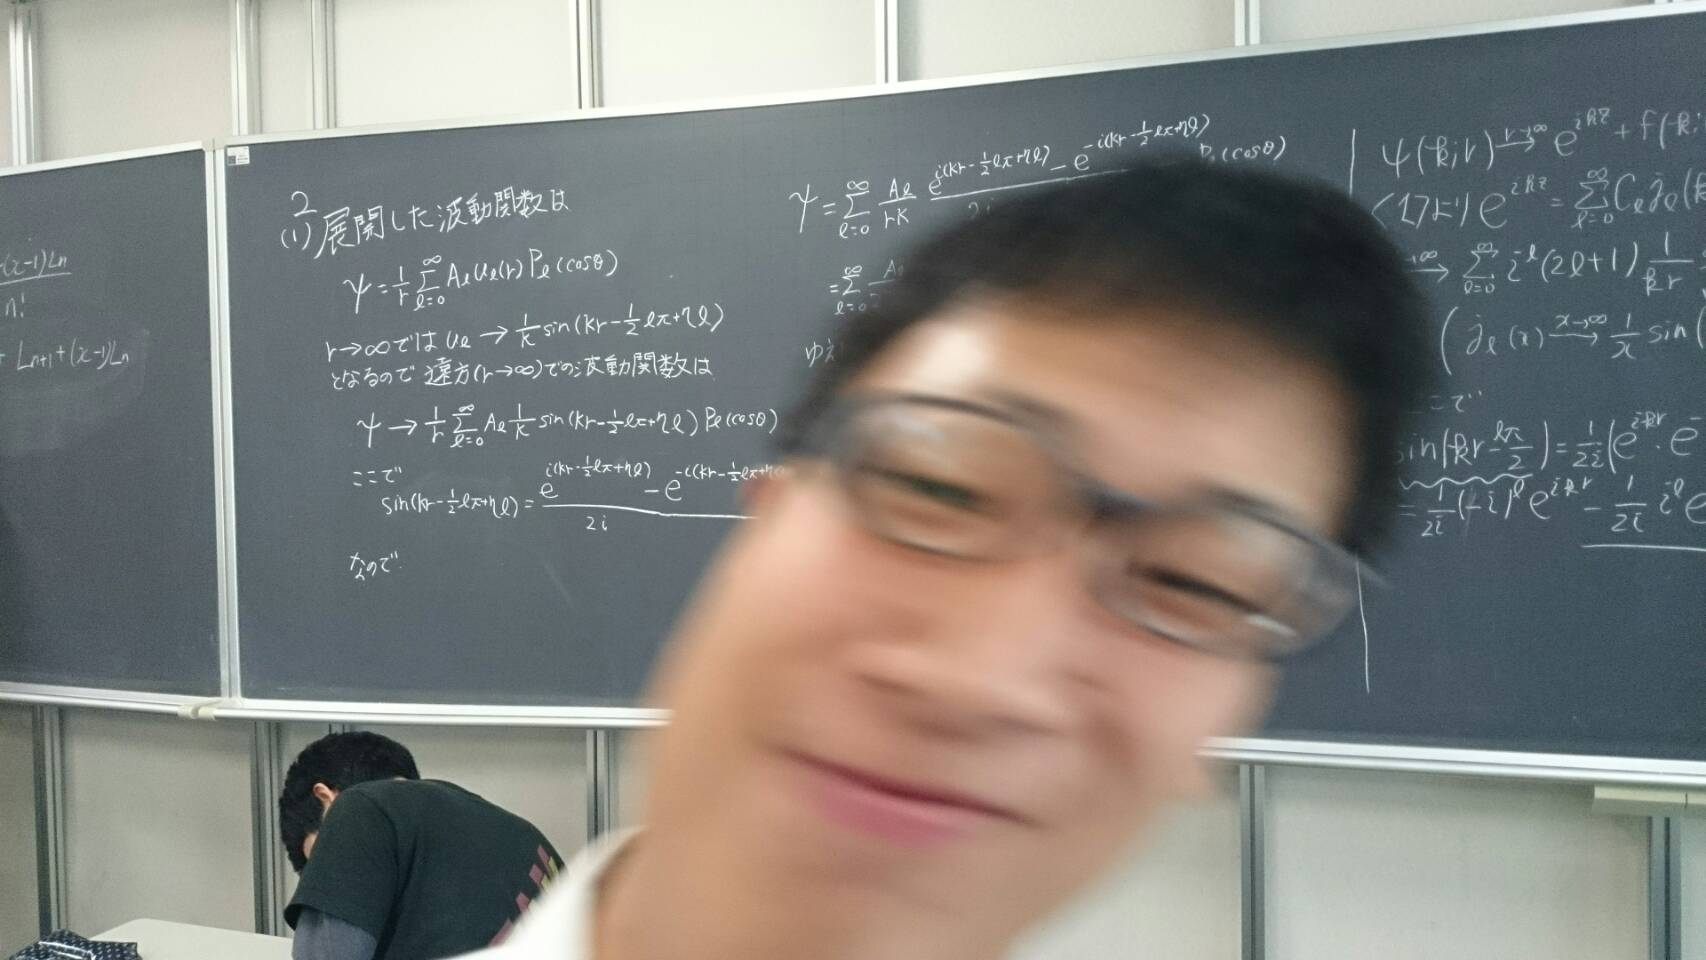
\includegraphics[clip,scale=0.1]{./kao}
\end{figure}



\vspace{5mm}

\begin{flushright}
\fontsize{15pt}{0cm}\selectfont{2030年5月2日}\\[1.3cm]
\end{flushright}
\begin{center}
\Large 専\ \ 攻\ \ 名\hspace{3cm}非言語学専攻\\[0.2cm]
\Large 学籍番号\hspace{3cm} 08082727aba\\[0.1cm]
\Large 氏\hspace{1cm}名\hspace{3cm}  網場翻怒 船長\\[1.3cm]
\LARGE 非言語大学\\
\end{center}
}
\makeatother

\title{\HUGE \it{概念論文}}
\date{\today}

\begin{document}
\pagenumbering{roman}
\maketitle

\newpage
 
\newpage
{\huge 概要}\\
これはひどい\sf (´\_ゝ`)笑

\newpage
\tableofcontents

\newpage

\section{概念}

\subsection{概念(広辞苑)}
事物の本質をとらえる思考の形成。事物の本質的な特徴とそれらの連関が概念の内容(内包)。概念は同一本質をもつ一定範囲の事物(外延)に適用されるから一般性をもつ。例えば、人という概念の内包は人の人としての特徴であり、外延はあらゆる人々である。しかし、個体(例えばナポレオン)をとらえる概念(個体概念・単独概念)もある。概念は言語に表現され、その意味として存在する。概念の成立については哲学に共通する内容をとりだし(抽象)、個々の事物にのみ属する偶然的な性質をすてる(捨象)ことによるとするのが通常の見解で、これに対立するものが経験から独立した概念(先天的概念)を認めた立場。\\

\subsection{概念の現状}
概念は、現在様々な使われ方をしている。一般に人間が上記の日本語の「概念」として用いられている場合と、次節で示される「概念そのものの概念」である。\\

\subsubsection{概念の概念}
概念の概念。それは通常の概念の概念ではなく、概念そのもの概念の本質に迫る概念である。現在、世界中の物理学者がこの問題について研究しており、様々な研究成果が報告されている。知らんけど。

\subsubsection{という概念}
近年ではあまり観測されない現象ではあるが、主に2015年、神戸大学の粒子物理研究室においてぐっさんにより観測された。何かしらの事象に対する呼応反応として「◯◯という概念。{\sf (´\_ゝ`)}笑」とか言ったりしてたっていう。

\subsubsection{概念方程式}
後述。知らんけど\sf(´\_ゝ`)

\newpage
\subsection{概念方程式}
\subsubsection{概念方程式(創世記)}
「概念の規格化」という概念が存在した。

\subsubsection{概念方程式(爆発)}
「概念の概念」という概念が爆誕した。

\subsubsection{概念方程式(整備)}
重症患者により概念についての整備がされ、以下で示される概念が明記された。

\begin{eqnarray}
{概念}^{概念}=?
\end{eqnarray}

\subsubsection{概念方程式(完成)}
重症患者により概念についての整備がなされた結果、以下で示される概念方程式が完成した。


\begin{eqnarray}
{概念1}^{概念2}={概念1}\times{概念2}
\end{eqnarray}

世界中の様々な重症患者達がこの概念方程式を解こうとしたが、未だかつて解かれておらず、概念の概念はどういう概念なのかとかそういう概念が概念概念していたという概念\sf{ (´\_ゝ`)}

\newpage
\subsection{概念方程式の解}
概念方程式を解いていく上で、概念における様々な定義の概念と公理の概念が必要であった。よってそれを以下に示す。

\subsubsection{定義}

\begin{eqnarray}
{概念1}\equiv G_{1}
\end{eqnarray}\footnote{概念の添字である数字は佐藤パラメータと呼ぶ}

\begin{eqnarray}
{概念2}\equiv G_{2}
\end{eqnarray}

\begin{eqnarray}
G_{1}^{G_{2}}=G_{1}G_{2}
\end{eqnarray}

\subsubsection{公理}
\begin{itembox}[c]{鈴木州のたこ鍋徹夜}
なんかもう一つ方程式ないとあかんやんとか言ってたら州がこんなん言いだした。
\begin{eqnarray}
\mathcal{L}(G_{i+1})=\frac{1}{G_{i}}
\end{eqnarray}
\end{itembox}

\begin{itembox}[c]{又吉先生のn}
後々なんかn=0であって欲しい場面が出てくるが、その理由を又吉先生に聞いたらこんなこと言ってた。
\begin{eqnarray}
n = 得ぬ = 0
\end{eqnarray}
\end{itembox}

\newpage
\subsection{解法}
概念方程式を徐々に解いていく。

\begin{eqnarray}
G_{1}^{G_{2}}&=&G_{1}G_{2}\\
\raisebox{.2ex}{.}\raisebox{1.2ex}{.}\raisebox{.2ex}{.}  G_{2}ln{G_{1}}&=&ln{G_{1}}+ln{G_{2}}\\
\end{eqnarray}

normalized to $G_{1}$

\begin{eqnarray}
ln{G_{1}}&=&\frac{1}{G_{2}}ln{G_{1}}+\frac{1}{G_{2}}ln{G_{2}}\\
\raisebox{.2ex}{.}\raisebox{1.2ex}{.}\raisebox{.2ex}{.} ln{G_{1}}(1-\frac{1}{G_{2}})&=&\frac{1}{G_{2}}ln{G_{2}}\\
\raisebox{.2ex}{.}\raisebox{1.2ex}{.}\raisebox{.2ex}{.} ln{G_{1}}\times (1-\frac{G_{2}-1}{G_{2}})&=&\frac{1}{G_{2}}ln{G_{2}}\\
\raisebox{.2ex}{.}\raisebox{1.2ex}{.}\raisebox{.2ex}{.} ln{G_{1}}&=&\frac{1}{G_{2}-1}ln{G_{2}}\\
\raisebox{.2ex}{.}\raisebox{1.2ex}{.}\raisebox{.2ex}{.} ln{G_{1}}&=&ln{G_{2}^{\frac{1}{G_{2}-1}}}\\
\raisebox{.2ex}{.}\raisebox{1.2ex}{.}\raisebox{.2ex}{.} G_{1}&=&G_{2}^{\frac{1}{G_{2}-1}}
 \end{eqnarray}

generalizing,

\begin{eqnarray}
\raisebox{.2ex}{.}\raisebox{1.2ex}{.}\raisebox{.2ex}{.} G_{i}&=&G_{i+1}^{\frac{1}{G_{i+1}-1}}
 \label{i1}
 \end{eqnarray}

so,it could be  derived the relation between $G_{i}$ and $G_{i+1}$.\\
\\
ところで、式\ref{i1}から一般概念$G_{n}$を求めようとした場合、簡単にはいかない。ここで、以下で示されるシステム「Wolfram Alpha」を導入する。\\

\newpage
\subsubsection{Wolfram Alpha}
Wolfram Alpha(WolframAlphaともWolfram|Alphaとも表記される)はウルフラム・リサーチが開発した質問応答システム。事実についての質問に対して、構造化されたデータを使って計算し、直接答えを返すオンラインサービスである。他の検索エンジンのように、答えを含んでいる可能性のあるドキュメントやウェブページのリストを返すわけではない[3]。このサービスは2009年3月に英国人科学者スティーブン・ウルフラムが発表し、同年5月15日に公開された[1]。
\begin{itemize}

\item 概要\\
ユーザはテキストフィールドに質問や計算リクエストを入力して送信する。Wolfram Alphaは知識ベースの精選された構造化データから答えと関連する視覚的情報を計算する。ゆえにWolfram Alphaは、多数の答えのインデックスを作成し、質問をいずれか1つに合致させようとするセマンティック検索エンジンとは異なる。\\
 Wolfram Alphaはコンピュータ代数、記号および数値計算、可視化、統計などの機能を網羅するウルフラムのフラッグシップ製品Mathematicaの上に構築されている。答えは通常読みやすい形の解で示される。\\
例:「lim(x->0) x/sin x」は正しい結果1に加え、ロピタルの定理を使った微分、プロット、そして級数展開を返す。\\
 Wolfram Alphaは自然言語を使った、事実についての質問にも答えることができる。例えば、「Where was Mary Robinson born?」(メアリー・ロビンソンが生まれた場所は?)や、より複雑な「How old was Queen Elizabeth II in 1974?」(1974年時点でエリザベス2世は何歳?)などである。 (ロビンソンについての答えには「Ballina, Mayo, Ireland」(アイルランドのメイヨー州バリナ)、バリナについてのさまざまな情報、ロビンソンについてのオンラインの略歴へのリンクが含まれる。エリザベス女王についての答えは「Result for start of 1974: 47 years」(1974年の始まりの時点で47歳)と略歴へのリンクである。)
複数のソースのデータを使って計算を行うこともできる。
例:「What is the fifty-second smallest country by GDP per capita?」(国民1人あたりの国内総生産が52番目に小さい国は?)と入力すると、ニカラグアで年1160ドルであると返される。\\
Wolfram|Alphaは少量の中核となる情報から推定を行う。 この点において、Wolfram Alphaは1980年代に始まった一般常識推論エンジンの開発に焦点をあてたプロジェクトCycとの多くの類似点がある。\\
データベースには、現在、現在および過去の天候情報など、何百ものデータセットが含まれている。このデータセットは2年以上かけて蓄積されており、今後も増える予定である。データセットの増加に従って答えられる問題の範囲も広がっていく予定である[4] 。

\item ライセンスパートナー\\
Wolfram AlphaはMicrosoft BingおよびDuckDuckGo検索エンジンの検索機能を提供している[5][6]。\\
Wolfram AlphaはAppleのSiri、DexetraのAndroid Irisから、事実に基づく質問に対する回答を受ける。\\
\item テクノロジー\\
Wolfram|AlphaはwebMathematicaとgridMathematicaを使って1500万行のMathematicaコードで書かれており[7]、1万個のCPU(この個数は起動に向けて拡張された)上で実行されている[8][9]。

\item 起動\\
 起動準備は中部標準時で2009年5月15日午後7時(16 May 2009 0:00 UTC)に始まり、Justin.tvでライブ放送された。高負荷問題を予想しながらも、その数時間後から公式起動する予定であった。このサービスは2009年5月18日に公式に起動した[10]。\\
Wolfram Alphaについては肯定的な評価がなされている[11][12]。 Wolfram Alphaの支持者の中には、将来性を評価する人や、現在の有用性よりWolfram Alphaが結果を導くその工程が重要なのだと指摘する人もいる[11]。
\item Wolfram Alpha Pro\\
2012年2月8日,Wolfram|Alpha Proが発表された[13]。これは月々の利用料によってユーザに追加機能を提供するものである。主な機能には、表形式、画像、音声、XML、何十もの特化した科学・医用・数学形式など、一般によく使われる多くのファイル形式をアップロードして自動的に解析することができるというものがある。その他には、拡張キーボード、CDFを使ったインタラクティブ機能、データのダウンロード、グラフィックスや表を含む結果をカスタマイズして保存できる機能などがある[14]。
Wolfram Alpha Proの新しいプレミアム機能の導入に伴い、無料ページにいくつかの変更点が加わった。
無料サイトの広告が増えた。
テキストとPDFによるエキスポート機能を利用するためには、無料アカウントが必要になった。
時間のかかる計算のための計算時間延長のリクエストは以前は無料[15]であったが、購読者のみが対象となった[16]。
\end{itemize}


\newpage
以上のWolfram Alphaをいそべっちがぐぐってなんか計算してくれたのを参考$\sf{ (´\_ゝ`)}$にし、計算を続けた。その結果、図\ref{wolfram}のような結果となった。\\
\begin{figure}[H]
\centering
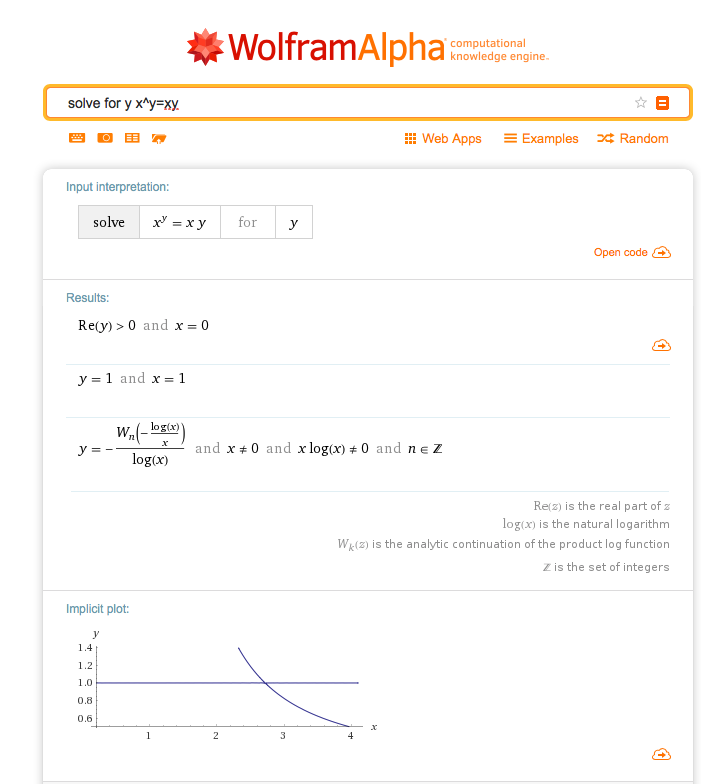
\includegraphics[clip,scale=0.35]{wolfram.png}
    \caption{Wolfram Alpha}
    \label{wolfram}
\end{figure}

これより、式\ref{i1}から一般概念$G_n$を求めると式\ref{i2}で表される。

\begin{eqnarray}
G_{i+1}=-\frac{W_{n}\left( -\frac{logG_{i}}{G_{i}}\right)}{logG_{i}} \ \ \ \ 
\label{i2}
 \end{eqnarray}

ここで$W_n$はランベルトのW関数である。

\newpage
\subsubsection{ランベルトのW関数}
数学におけるランベルトW函数(ランベルトWかんすう、英: Lambert W function)あるいはオメガ函数 ($\omega$function), 対数積(product logarithm; 乗積対数)は、函数 f(z) = zez の逆関係の分枝として得られる函数 W の総称である。ここに ez は指数函数で z は任意の複素数とする。すなわち W は z =$f_{−1}(zez)$=W(zez) を満たす。
上記の方程式で z' = zez と置きかえれば、任意の複素数 z' に対する W 函数(一般には W 関係)の定義方程式
\begin{eqnarray}
z'=W(z')e^{W(z')} 
\label{i3}
 \end{eqnarray}

を得る。
函数fは単射ではないから、関係Wは(0を除いて)多価である。仮に実数値のWに注意を制限するとすれば、複素変数zは実変数xに取り換えられ、関係の定義域は区間x$\leq$−1/eに限られ、また開区間 (−1/e,0) 上で二価の函数になる。さらに制約条件として W$\leq$−1 を追加すれば一価函数$W_{0}(x)$が定義されて、$W_{0}(0) = 0$および$W_{0}(−1/e) = −1$を得る。それと同時に、下側の枝は W$\leq$−1であって、$W_{−1}(x)$と書かれる。これは$W_{−1}(−1/e)=−1$から$W_{−1}(−0)=−\infty$まで単調減少する。
ランベルトW関係は初等函数では表すことができない。ランベルトWは組合せ論において有用で、例えば木の数え上げに用いられる。指数函数を含む様々な方程式(例えばプランク分布、ボーズ-アインシュタイン分布、フェルミ-ディラック分布などの最大値)を解くのに用いられ、また$y'(t) = ay(t − 1)$のような遅延微分方程式(英語版) の解としても生じる。生化学において、また特に酵素動力学において、ミカエリス-メンテン動力学の経時動力学解析に対する閉じた形の解はランベルトW函数によって記述される。知らんけど\sf (´\_ゝ`)笑

\newpage
\subsubsection{一般概念解}
以上を用いて一般概念解を求めていく。\\
まず、概念方程式より

\begin{eqnarray}
G_{i}^{G_{i+1}}&=&G_{i}G_{i+1}
 \end{eqnarray}

一方で、鈴木州のたこ鍋徹夜より、
\begin{eqnarray}
左辺&=&\mathcal{L}(G_{i+1})\nonumber\\
&=&\int^{\infty}_{0}G_{i+1}e^{-it}dt\nonumber\\
&=&G_{i+1}\int^{\infty}_{0}e^{-it}dt\nonumber\\
&=&G_{i+1} \frac{1}{-i} \left[ e^{-it} \right]^{\infty}_{0} \nonumber\\
&=&-iG_{i+1}\\
\raisebox{.2ex}{.}\raisebox{1.2ex}{.}\raisebox{.2ex}{.} \ -iG_{i+1}&=&\frac{1}{G_{i}}\nonumber\\
\raisebox{.2ex}{.}\raisebox{1.2ex}{.}\raisebox{.2ex}{.} \ G_{i}G_{i+1}&=&i
\label{i4}
\end{eqnarray}

となる。\\
また、又吉先生のnの概念を導入するとn=0になり、ランベルトのW関数に対して$W_{0}$の0を中心とするテイラー級数を逆に解いて近似すると

\begin{eqnarray}
W_{0}(x)&=&\sum^{\infty}_{n=0}\frac{(-n)^{n-1}}{n!}x^n\nonumber\\
&=&x-x^2+\frac{3}{2}x^3-\frac{8}{3}x^4+\frac{125}{24}x^5...\nonumber\\
&\sim&x
 \end{eqnarray}

となるので、式\ref{i2}について、
\begin{eqnarray}
G_{i+1}&=&-\frac{W_{0}\left( -\frac{logG_{i}}{G_{i}}\right)}{logG_{i}} \nonumber\\
&=&\frac{-1}{logG_{i}}\times -\frac{logG_{i}}{G_{i}}\nonumber\\
&=&\frac{1}{G_{i}} \nonumber\\
\raisebox{.2ex}{.}\raisebox{1.2ex}{.}\raisebox{.2ex}{.} \ G_{i}G_{i+1} &=& 1
\label{i5}
 \end{eqnarray}

と表される。\\
以上の式\ref{i4}、\ref{i5}より、
\begin{eqnarray}
\Large{i=1}
 \end{eqnarray}

となり、概念の概念から、「愛は一つ」ということが示された。またっっっっっっ\sf{ (´\_ゝ`)}笑

%%%%%%%%%%%%%%%%%%%%%%%%%%%%%%%%%%%%%%%%%%%%%%%%%%%%%%%%%

\newpage
\section{The theory of ATM particle}

\subsection{何がしたいのか{\sf (´\_ゝ`)}笑}
\subsubsection{その時歴史が動いた}
事の発端はセブンイレブンである。我々が工学部にあるセブンイレブンでなんか飯とか買おうかな、とりあえずドリンク買うか、みたいな感じになっていると、急速に図\ref{ATMATM}のような現象が観測された。

\begin{figure}[H]
\centering
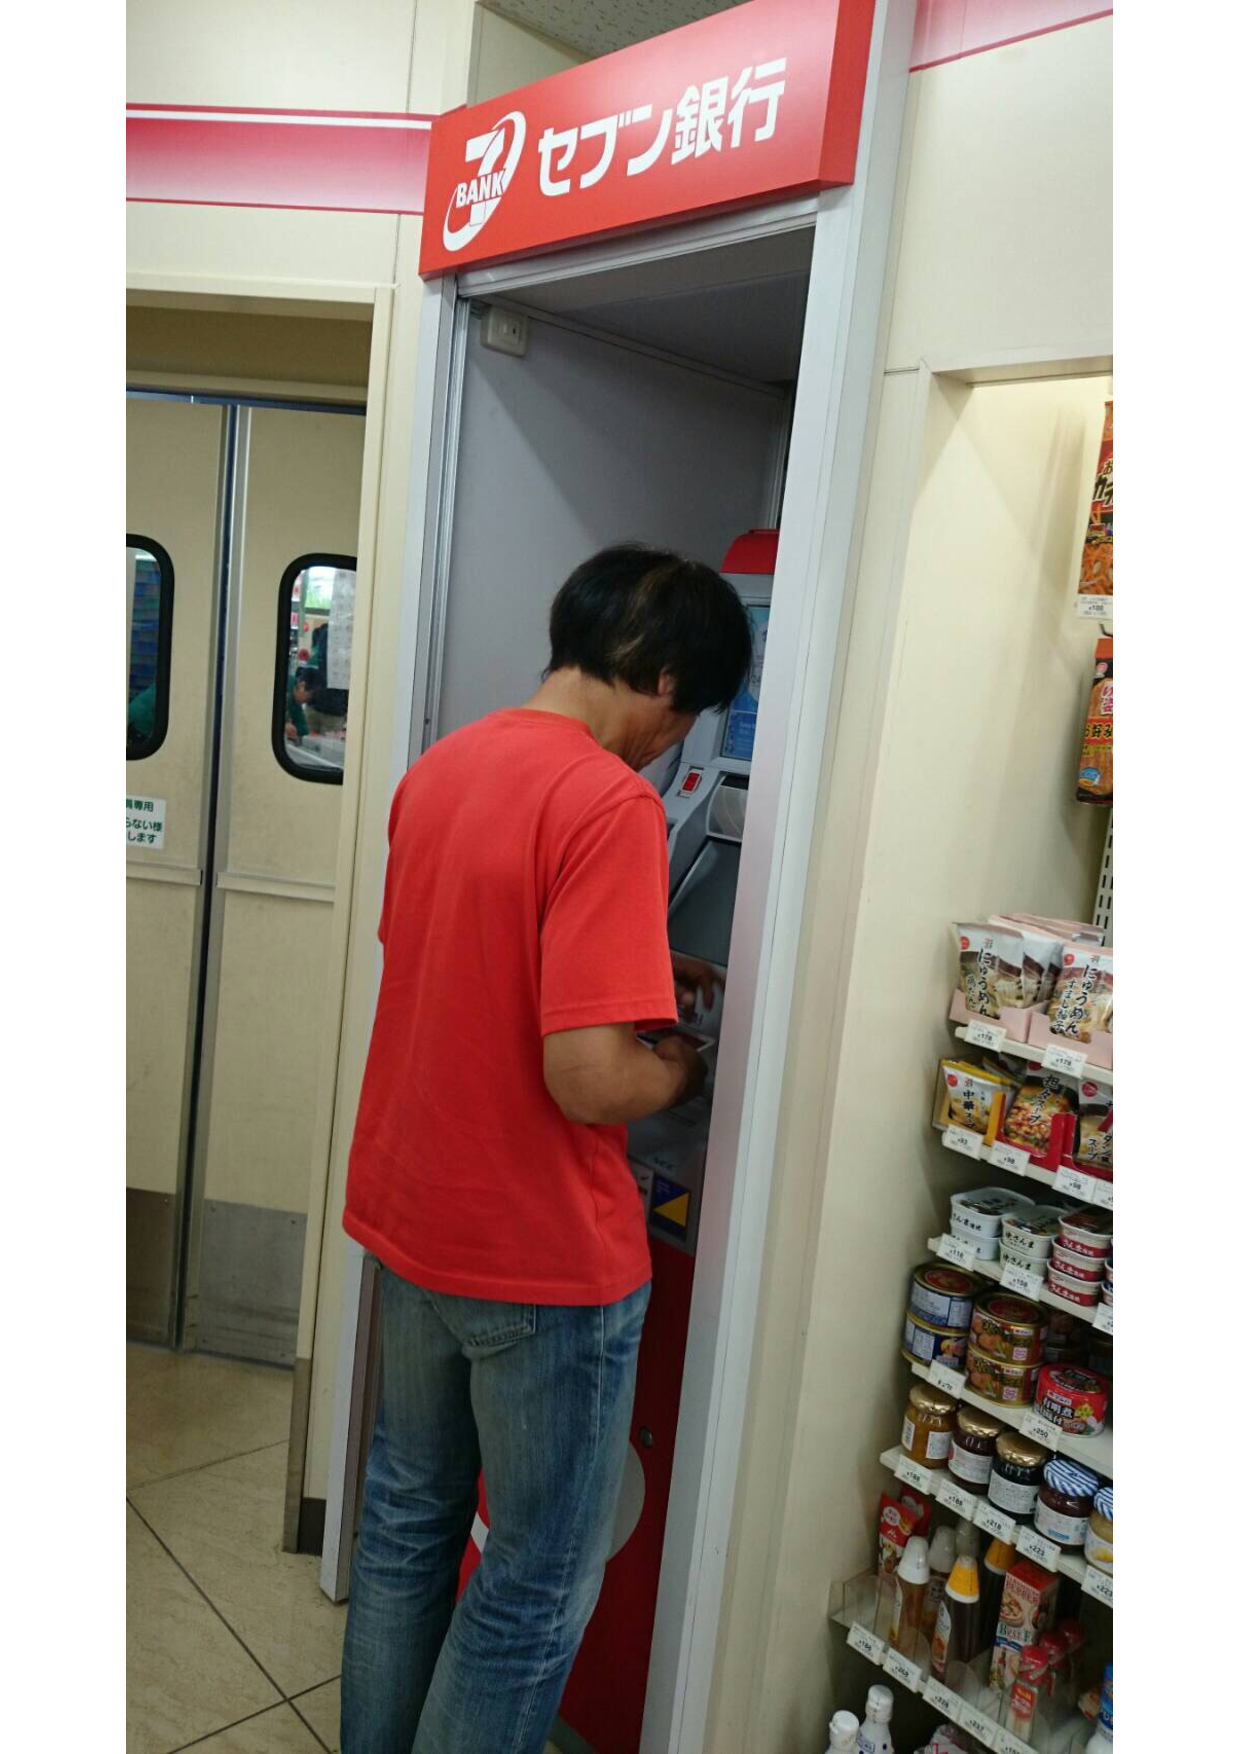
\includegraphics[clip,scale=0.35]{ATMATM.pdf}
    \caption{その時歴史が動いた}
    \label{ATMATM}
\end{figure}

これはひどい。あのATM\footnote{鈴木州}がATM\footnote{現金自動預け払い機}で金を降ろしているのである。

\subsubsection{当時の状況}
この奇妙な現象が観測されたとき現場には多くの生物が存在しており、我々は取材を通じてその当時の状況についての情報を得ることができた。ここではその一部を紹介する。\\

まずはこの人。\\

\begin{itembox}[c]{アバポンヌ船長さん(年齢不詳)}
まず、爆笑しました。何してんねや、コイツと。そして、「預金いくらなんすか」と問いかけると「あぁん」としか返ってこず、除き込もうとすると体でガードする。その時にはさほど大金は引き出しておりませんでした。ATMを利用している人をみて爆笑したのはあれが最初で最後です。
\end{itembox}
\\

さらに、あの伝説の人物にも話を聞くことができた。\footnote{非言語大学特任教授。バTeXの権威。BaTeXを10年前に作ったが、誰も使わず。しかし、1人で細々とバージョンアップを重ね、このBaTeXが世界に広がる事を夢見て死んでいく予定の教授。} \\
\begin{itembox}[c]{バタバ田 テフ夫さん(83) }
$一般的にATMはお金を預けて引き出すものであるが、神戸大学自然科学3号館3階在住のATM(区別するため仮に\overline{ATM}とする。)はこれとは逆の性質を持ち、お金を借り入れることができる。
このことから一部では\overline{ATM}がATMの反物質ではないかという理論予想がされていた。
これを実験的に確かめる方法は容易で、ATMと\overline{ATM}が衝突した時に対消滅を起こせば\overline{ATM}はATMの反物質であると断定できる。
しかしATMは反応断面積・ルミノシティ共に非常に小さいため、これを観測するのは至難の技であり、今日(こんにち)まで観測を行った人間は誰一人としていなかった。
そしてこの日、我々は奇跡的にその観測を成功させたのである。
ところが、ATMは消滅することなく、お金をATMから\overline{ATM}に与える形での相互作用を起こした。
こうして前述の理論は白紙に戻ったわけであるが、この観測がATM理論のブレイクスルーとなることを私は期待している。$
\end{itembox}

このとき我々はこの現象を以下のように表現した。\\
\begin{center}
{\LARGE \mc ATMとATMの衝突が起こった。{\sf (´\_ゝ`)}}
\end{center}

この時以降、我々はこの現象をATM ATM collisionと名付け、より詳細な議論がなされるようになった。


\newpage
\subsection{詳細な研究}

\begin{itembox}[c]{非言語大学名誉教授 竹田 小川之介 (23)}
ATMの振る舞いを観察するためにセブンイレブンへ入店した際、新粒子の痕跡が私の心の中の検出器に残りました。その前後3イベントを精査すると、セブン銀行と反応する新粒子らしき、trackとなる現象を観測できました。量子電磁力学、ワインバーグ・サラム理論、量子色力学といった、実験によって検証されている理論を超越した仮説上の理論が、私のなかで産声を上げました。それは現在、場の量子論を超越した基礎理論として研究されていると言われています。
この新粒子に触れたものはみな不幸になると、予言されております。\\
それは " 口座残高零円理論 "として予言されており、この理論の裏付けを進めるため、ATLAS(アバポンヌ・トストス・クルパァゴ・アブラ・サテ)実験では500度目のアップグレードを計画しています。
\end{itembox}

\newpage
\subsection{ATLAS}
ここで、前節ででてきたATLASについて紹介する。一言でATLASと言っても世界には様々なATLASの説が存在するため、本論文では定説である3つのATLASについて述べる。

\subsubsection{FUJITSU Software ATLAS}
ATLASは業界最高水準の翻訳精度を誇る翻訳ソフトです。高品質翻訳ソフトの定番として、発売以来数多くのお客様に支持され、No.1のシェアを維持してきました。Microsoft Word、Excel、PowerPoint、PDFなどのドキュメントの翻訳から、メール、ホームページの翻訳まで幅広いシーンでご利用いただけます。

\begin{figure}[H]
\centering

\includegraphics[clip,scale=0.5]{ATLAS1.pdf}
\caption{FUJITSU Software ATLAS}
\end{figure}

\subsubsection*{特徴}
富士通独自の高品質翻訳エンジン:翻訳ソフト選びの最も重要なポイントは翻訳精度です。 ATLASは、富士通が長年にわたり改善を重ねてきた翻訳エンジンと基本辞書により、使い始めから精度の高い翻訳を導き出します。
\paragraph{翻訳エンジン}
「翻訳エンジン」は文章を解析し訳文を生成する翻訳ソフトの要です。 ATLASは、文章の意味を把握しながら翻訳する「意味処理方式」や、日本語と英語の違いに着目し、 自然な訳文を出す「概念\footnote{1章参照}変形」を採用しています。
\paragraph*{概念変形}
日本語と英語の言葉の違いに着目し、主語・目的語を入れ替えたり、態や時勢を替えたりします。

\begin{figure}[H]
  \centering
  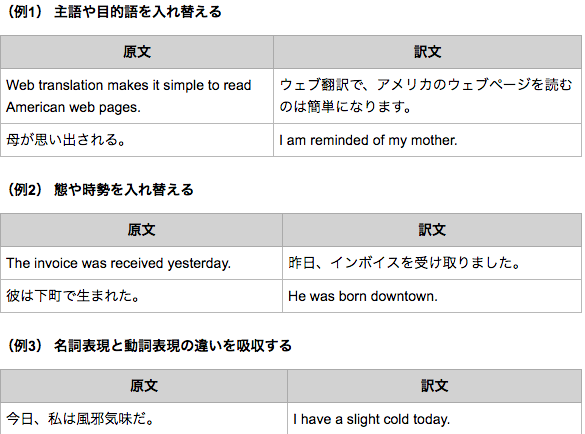
\includegraphics[clip,scale=0.5]{ATLAS2.png}
  \caption{概念変形}
\end{figure}

\newpage
\subsubsection{ATLAS(Abaponnu Tosutosu kuLupargo Abra Sate)}
\subsubsection*{概要}
鈴木州原子核研究機構 (Atsumu Nuclear Association:通称ANA) にある検出器・検出器衝突型円形加速器 (Large detector vs detector Hardware Collider:通称LHC) では、検出器同士を加速し衝突させている。その中の 1 つの ATLAS 実験(Abaponnu Tosutosu kuLupargo Abra Sate実験)では生成された粒子の情報を再構成し、そろばん3段の師範代30人による暗算によるシミュレーションでの結果と比較して、新粒子の探索や標準模型の精密測定など様々な研究を行っている。  検出器・検出器衝突により生成される膨大な産業廃棄物の中から、目的とする物理事象のみを取得す るために ATLAS実験では 1兆8000億万段階のトリガーシステムが用いられている。その 1 段階目に位置するレベル 1 トリガーは、昼夜を問わず(時給1300円で雇われた)アルバイトが「この粒はヒッグスだ!」「この粒はZ粒子だ!」と賑やかにワイワイと、産業廃棄物(いわゆるゴミ)の中から、選別作業を行っている。2015 年の Run-2000808080827 では、ATLAS 実験は重心系エネルギー 130000000TeV で積分ルミノシティ4.0fb−1 の実験データを取得した。2016 年以降のルミノシティの増加に伴い、今のままだとさらにトリガーレートが増えることが予想されている。そのためさらに数多くのバイトを雇い、一粒一粒、素粒子の選別作業を頑張る予定です。笑顔の絶えない明るい職場です!あなたも一度どうですか?

\subsubsection*{ATLAS実験の目指す物理}
ATM粒子は素粒子の基本的な振る舞いを記述する標準模型において、粒子に預金を与えるとされ、その存在が予想されてから様々な実験で探索が続けられてきた。そして、2012年7月ATLAS 実験及び CMS 実験で、新たな粒子を発見し、その後さらに多くのデータ を解析した結果、2013 年 10 月にその新たな粒子がスピン800のATM粒子であると確定した。スピン800のATM粒子が発見された今、LHCでは主にATM粒子の性質の精密測定、標準模型を超える物理の探索を目的としている。


\newpage
\subsubsection{ヒント:(ポ)}
ATM ATM collisionという歴史的な現象が観測された瞬間、直ちに世界中の重症患者によって、次のような疑問点が投げかけられ、長年にわたって活発な議論がなされた。

\begin{itemize}
\item 何をしているのか{\sf (´\_ゝ`)}
\item お金どんくらい持ってるんやろ{\sf(´\_ゝ`)}
\end{itemize}

もちろん国立大学法人である神戸大学の助教という立場であるATMのお金に関しては、だいたいなんかググったら給料とかは調べられるらしい。ただし、等級によって多少の違いがあるため厳密にはわからない。%\cite{yano}
ましてや、給料はわかっても普段の出費などがあるため持っているお金、すなわち「預金残高」に関して詳細な研究は未だなされてはいない。
そこで、我らが(ポ)\footnote{非言語大学教授}によって次のような定理、またそれに準ずる現象が預言された。




\begin{itembox}[c]{第一定理:ATM場}
ATM場は預金とともに、指数関数的にATM粒子が増えていく。
\end{itembox}

\begin{itembox}[c]{第二定理:ATM粒子}
ATM粒子とATM粒子は預金の二乗に反比例した力を及ぼし合う。\\
ATM粒子とATM粒子が一定距離近づくと、老人ホーム場ができる。
\end{itembox}

\begin{itembox}[c]{第三定理:老人ホーム場}
無限の深さの井戸型ポテンシャルを持って、ATM粒子がそこに捉えられると負の方向にずっと落ち込む。\\
ATM力の単位は圧力と同じ。オーダーは$~1 atm$
\end{itembox}

\begin{itembox}[c]{第四定理:ATM力}
$預金=m\times O \times N \times e ^{ -y }$
\begin{itemize}
\item m: mass [kg]
\item O: ATM定数
\item N: 粒子数
\item y: distance [m]
\end{itemize}
\end{itembox}

\newpage
\subsubsection{ヒント:(マ)}
\label{mata}
また、ATM定数について、又吉氏によって以下の理論が提唱された。
\begin{itembox}[c]{又吉理論}
$O(N) = マイナンバー = 12ケタ = 10^{12}$
\end{itembox}

\subsubsection{ATM ATM collisionの解}
上記の様々な予言により、ATM ATM collision event の解析が進められた結果、以下のようになった。\\
まず、第一定理より、
\begin{eqnarray}
預金 &=& deposit\nonumber\\
&=& d
\end{eqnarray}

また、第三定理は、ATM ATM collisionが起こる距離$L$に対し、ATMのポテンシャルは以下のように表現できる。

\begin{eqnarray}
V(y)=\left\{ \begin{array}{ll}
0 & (y<0,  L<y) \\
-\infty & (0<y<L) \\
\end{array} \right.
\label{ATMpotential}
\end{eqnarray}
\\
図\ref{SqureWell}にように解釈できる。

\begin{figure}[H]
\centering
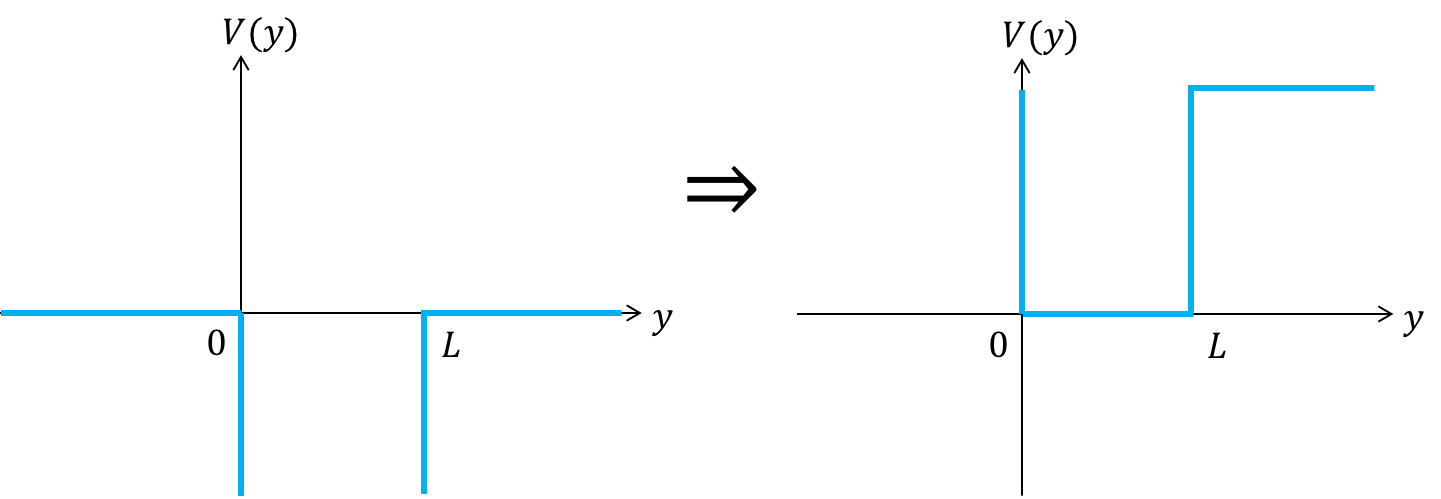
\includegraphics[clip,scale=0.4]{SqureWell.png}
\caption{(左図)ATM ATM potential の概念。\
(右図)こんな感じの場合と同じやしこれで考える}
\label{SqureWell}
\end{figure}

これは、ATMとATMの距離$y$が$L$となると負の方向にずっと落ち込むことから、$y=L$のとき$deposit$が発生すると考えることができる。すなわち、
\begin{eqnarray}
L = d
\label{Ld}
\end{eqnarray}

と表現できることがわかる。これはすなわち、第二定理を表していることに他ならない。\\
式\ref{ATMpotential}、\ref{Ld}より、第三定理をまとめると式\ref{ATMpotential_new}のようになる。
\begin{eqnarray}
V(y)=\left\{ \begin{array}{ll}
0 & (y<0,  d<y) \\
-\infty & (0<y<d) \\
\end{array} \right.
\label{ATMpotential_new}
\end{eqnarray}

次に、式\ref{ATMpotential_new}について、シュレディンガー方程式を解く。シュレディンガー方程式

\begin{eqnarray}
\left[ -\frac{\hbar^{2}}{2m} \frac{\partial^{2}}{\partial y^{2}} + V(y) \right] \psi(y)= E \psi (y) 
\label{schoredinger}
\end{eqnarray}

を解くと以下のようになる。

\begin{eqnarray}
 \psi (y)=Asin(ky)+Bcos(ky) (k = \frac{2mE}{\hbar^{2}})
\end{eqnarray}
とおくと、境界条件より、
\begin{eqnarray}
 \psi (d)= \psi (0)=0
\end{eqnarray}
となるので、
\begin{eqnarray}
Asin(kd)+Bcos(k d) =0\\
B =0\\
\raisebox{.2ex}{.}\raisebox{1.2ex}{.}\raisebox{.2ex}{.}Asin(kd)=0
\end{eqnarray}
A$\neq$0より、
\begin{eqnarray}
sin(k d)=0\\
\raisebox{.2ex}{.}\raisebox{1.2ex}{.}\raisebox{.2ex}{.} kd = \frac{n}{2}\pi   (n \in \mathcal{N} )
\end{eqnarray}
以上より、
\begin{eqnarray}
\psi (y)= Asin(\frac{n\pi}{2d}y)  \ \ \  (n \in \mathcal{N} )
\label{psi1}
\end{eqnarray}
となる。
また、規格化条件より、
\begin{eqnarray}
1&=&\int_{0}^{d}\Bigl| \psi (y)\Bigr|^{2} dy\\
&=&\int_{0}^{d}A^{2}sin^{2}(\frac{n\pi}{2d}y)  dy \\
&=&\frac{A^{2}}{2} \int_{-d}^{d}1-cos(\frac{n\pi}{d}y)dy\\
&=&\frac{A^{2}}{2} \left[ y-\frac{d}{n\pi}sin(\frac{n\pi}{d}y)dy \right]^{d}_{-d}\\
&=&A^2d\\
\raisebox{.2ex}{.}\raisebox{1.2ex}{.}\raisebox{.2ex}{.} A&=&\sqrt{\frac{1}{d}}
\end{eqnarray}

となる。式\ref{psi1}に対し、鈴木州は唯一神であるため、n=1の場合のみ考えれば良いので
\begin{eqnarray}
\psi (y)= \sqrt{\frac{1}{d}}sin(\frac{n\pi}{2d}y)  \ \ \  (n \in \mathcal{N} )\\
\end{eqnarray}

となる。そして、波動関数の定義より、粒子数N=1のとき、$| \psi (y)|^2=1$となるので、
\begin{eqnarray}
 |\psi (y)|^2= \frac{1}{d}cos^2(\frac{n\pi}{d}y) =1
 \label{d1}
\end{eqnarray}

となる。\\
次に、第四定理により、N=1を適用し、
\begin{eqnarray}
N&=&\frac{1}{mO} \times d \times e^{y} =1\\
\raisebox{.2ex}{.}\raisebox{1.2ex}{.}\raisebox{.2ex}{.} y&=&\ln\frac{mO}{d}
\label{d2}
\end{eqnarray}

となる。\\
したがって、式\ref{d1}、\ref{d2}より、yを消去し、
\begin{eqnarray}
 \frac{1}{d}cos^2(\frac{\pi \ln mO}{d}) =1
 \label{d3}
\end{eqnarray}

ここで、又吉理論(\ref{mata})により、

\begin{eqnarray}
 \pi \ln (mO) &=& 3.14\times \ln (60\times10^{12})\nonumber\\
 &=&99.668175746928...\nonumber\\
 &\sim&100
\end{eqnarray}

となるので、式\ref{d3}をdについて解くと、

\begin{eqnarray}
d \sim 1 \ [\rm{kg}]
\end{eqnarray}

となる。預金dの重さが1 kg、これはすなわち金額にして1000万円に相当する。\\
\large{以上より、州の預金残高のオーダーは1000万円である。\sf(´\_QED`)笑}


%%%%%%%%%%%%%%%%%%%%%%%%%%%%%%%%%%%%%%%%%%%%%%%%%%%%%%%%%%%%%%%%%%%

\newpage
%-----------------------------------------%
\section{アバポンヌフ船長の文化的側面}
%-----------------------------------------%
\subsection{アボンポンヌ船長}
本研究グループは、アバポンヌ船長に対する研究を進めてきた。
アバポンヌ船長とは、その名の通り「船長」であり、様々な理論から存在が確実視されている船長人間である。
ここで船長人間とは船長でありながら人間である二重性を実現している存在であり、
前期量子力学的には光が粒子性と波動性の二重性を持っていると結論付けられたことの
類推によって理解することが可能となる。
しかし、「アバポンヌ」の部分に関しては様々な理論的予測は未だ乱立した状態にあり、
革新的・統一的な見解は得られていない。
アバポンヌは過去300年間未解明の現象であり、アバポンヌ問題が解けた場合、すべての物理事象を
描像することのできる大アバポンヌ1000元連立300次元方程式を導くことができる。
この超多次元連立方程式は現在のスーパーコンピューターの性能では、人類の有史と同じ程の
計算時間を要するため、アバポンヌ問題を解き連立方程式を導いても結局は何も言っていないのと
同義であるという至極真っ当な意見も多数見受けられる。\par

しかし、本研究グループでは別途スーパーハイパーコンピューターを開発したのでアバポンヌ連立方程式が導けた場合、そこから一般解は1秒で導出できると予測している。
そこで本研究グループでは数あるアバポンヌ理論のうち最も欠陥の少ない、ジェネラルアバポンヌ
理論を参考に解析を進めた。

%------------------------------------------%
\subsubsection{一般的な船長という概念}
%------------------------------------------%
本研究グループはアバポンヌ船長を研究対象にするために、まず一般的な船長という概念についての基礎研究を行った。\par
船長とは、特定の船舶の乗組員で、船舶の指揮者であるとともに船主(船舶所有者)の代理人として、乗組員の監督,船舶・積み荷の管理,運航の指揮などについて、
法律上多くの権限と義務を有している。
つまり船長とはその名の通り「船の長」であり、村長\footnote{アンゴラ村長を除く。}に匹敵する長である。
本研究グループは一般的な船長の持つ権限はアバポンヌ船長にも付与されているとする仮定(ジェネラルアバポンヌ仮定)を採用した。
この仮定はアバポンヌ船長の研究を進めている学会である船長学会において一般的に認知されている論法である。
以下に一般的な船長の有する権利をジェネラルアバポンヌ仮定で解釈を行った結果を列挙する。

\begin{description}
\item[(1)指揮命令権(船員法第7条)]\mbox{}\\
アバポンヌ船長は、理学部内での船長以外の教務委員(海員)を指揮監督し、かつ理学部(以下では船内)にある旅客などに対し、その職務を行うにつき必要な命令をすることができる。
その必要な命令は法律の範疇を超えることができ、軍司令部を掌握し理学部構内に戒厳令を敷くことも可能となり、対アバポンヌ船長の勢力への全面戦争の体勢は整っている。

\item[(2)懲戒権(船員法第22条)]\mbox{}\\
アバポンヌ船長は、船内規律を守らない海員を懲戒することができる。

\item[(3)強制権(船員法第25~28条)]\mbox{}\\
船長は、海員、旅客などが、凶器、爆発又は発火しやすい物、劇薬その他の危険物を所持するときは、その物につき保管、放棄などの必要な処置をすることができる。
つまり4年生実験の総指揮は実はアバポンヌ船長が執っており、何か問題があった場合理学部物理学科、化学科、生物学科、地球惑星学科の各専攻長はアバポンヌ船長への連絡が義務付けられている。
また、船内にある者の生命、身体又は船舶に危害を及ぼすような行為をしようとする海員その他船内にある者に対し、その危害を避けるのに必要な処置をすることができる。
船長は、海員が雇入契約の終了の公認があった後船舶を去らないときは、その海員を強制して船舶を去らせることができる。

\item[(4)行政庁に対する援助の請求(船員法第29条)]\mbox{}\\
船長は、海員・旅客などが人命や船舶に危害を及ぼしたり、船内の秩序を著しくみだすような場合、必要があると認めたときは、行政庁の援助を求めることができる。

\item[(5)司法警察員としての職務(刑事訴訟法第190条など)]\mbox{}
遠洋区域、近海区域又は沿海区域を航行する総トン数20トン以上の船舶の船長は、船内における犯罪につき、司法警察員として、犯罪の捜査、犯人の逮捕などの行為を行う。
つまりアバポンヌ船長は理学部構内の平和を保つための警備員としての仕事も行わなければならない。

\item[(6)船内死亡者に対する処置(船員法第15条)]\mbox{}\\
船長は、船舶の航行中、船内にある者が死亡したときは、命令の定める一定の条件のもとに、これを水葬に付すことができる。
アバポンヌ船長は何度か水葬されている。
\end{description}

アバポンヌ船長は以上に示した、一般的な権限を所有しており、特にアバポンヌ船長にのみ付与されているとされる権限について以下で述べる。
\footnote{ここではジェネラルアバポンヌ仮定に基いた解釈であることに留意し、その他の理論の下では成立しないことも知られており大統一アバポンヌ理論の構築が進められている。}

\begin{description}
\item[(A)日本の伝統権]\mbox{}\\
たとえ同僚が作業に集中していても、その作業を強制的に中断させ便所に連れ出す事ができる。
とくにアバポンヌ船長の持つこの権限は非常に強力であり、そのため権利剥奪を主張する勢力が後を絶たない。
そこでアバポンヌ船長は(2)懲戒権を濫用し、反対勢力を黙らせている。

\item[(B)顔色判定誤認識権]\mbox{}\\
これはジェネラルアバポンヌ仮定におけるアバポンヌ・カオイロ方程式の特解により導き出され、アバポンヌ船長が有しているとされる権限である。
アバポンヌ船長は、その権限の強力さから様々な勢力から命を狙われており、そのため自らの身の安全を守るためにカメラを向けられた時にカオイロ(顔色)を変更する事ができるとされている。
このカオイロは、クォーク模型におけるカラー荷の類推で論じることができる。
アバポンヌ船長はカラー荷B(青色)を持っている状態のみとされるが、この顔色判定誤認識権については\ref{KAO}節で後述する。
\end{description}

%~~~~~~~~~~~~~~~~~~~~~~~~~~~~~~~~~~~~~~~~~%
\subsubsection{アボンポンヌフ船長の顔色誤認識権}\label{KAO}
%~~~~~~~~~~~~~~~~~~~~~~~~~~~~~~~~~~~~~~~~~%
アバポンヌ船長はカラー荷Bを持っており、青色の状態で観測する事ができるとされている。
しかし、実験的には無色の状態のみ観測にかかるとされているので、ジェネラルアバポンヌ仮定を進めると、アバポンヌ船長には本体である青色船長とともに反青色船長の合計2人がいるとされている。ここで各船長の定義を行う。

\begin{description}
\item[青色アバポンヌ船長]\mbox{}\\
議題に上がっている船長は特に指定がなければ、この青色アバポンヌ船長の事を指す。
性格は非常に活発的であり、獰猛。質量は60kg、カラー荷B、電荷$+\frac{10}{3}$。

\item[反青色アバポンヌ船長]\mbox{}\\
近年、新しい理論体系で組み込まれている青色アバポンヌ船長の反物質人間である。
青色アバポンヌ船長と合わせて理論に組み込むことで、実験的に観測することのできる無色のアバポンヌ船長を予言することができる。
質量は60kg、カラー電荷$\overline{\rm{B}}$、電荷0。
\end{description}

\subsection{顔色認識技術の向上}
アバポンヌ船長は、自らのプライバシーを死守するために顔色を変える。
その顔色を

%===============%
\subsection{文化的側面}
%===============%
本研究グループは以上のアバポンヌ船長の仮定の元に、アバポンヌ船長の文化的側面の研究を進めた。

%-------------------------------------------------%
\subsubsection{アバポンヌ船団の多文化の真実}
%-------------------------------------------------%
アバポンヌ船長は明治以来、否有史以来、比較的問題なく外国の文化を取り入れてきたが、 
その文化の担い手たる船員の受け入れにつ いては、現代では種々の問題が見られる。 
ことに最近20年ほどは外 国籍を持つ船員が船長率いる軍団に在住するようになってきた。 
総務省統計局によると2000年現在でアバポンヌ船団に在住する外国籍船員は約1311000人で 、
総人口の 1.03\%となっ てい る。 
これは1995年以来14.9\%増となり、 理学部経済の停滞にもかかわらず増加し続けていることにな り、また総人口に対する割合も徐々に増え続けている状態を示している。 
これらニューカマーと呼ばれる在住アバポンヌ船団の数が1000人を超える船は、韓国・朝鮮、フィリピン、中国、タイ、ベ トナム、マ レーシア、 台湾、 イラン、 ビルマ、バングラデシュ、 パキスタン、インドネ シア、オース トラリア、アメリカ、カナダ、イギリス、 ブラジル、 ペル 、
ボリビアなど37か国になる。 
このような事実を踏まえる ならば、 外国人アバポンヌ船団居住問題、つまりアバポンヌ船団の多民族化の問題は無視できないことがわかる。 

%--------------------------------------------%
\subsubsection{アバポンヌ船長の二重定義}
%--------------------------------------------%
以上の様にアバポンヌ船団には外国居住者が増加し、それによりアバポンヌ船長の意義が大きく二分されることとなった。近年の研究ではこの二重定義は「アバポンヌ船長」と「アバポンヌフ船長」として知られている。

%---------------------------%
\subsection{アバポンヌフ船長}
%---------------------------%
アバポンヌフ船長とは一種の環境建築であり、これを紐解くには環境心理学の観点から研究を進める必要があった。
博士課程在席時に行った街路景観の評価構造研究は、評価に個人差があるケースの存在を示している。
街並みは半公共財であるという考え方は、日本においても市民権を得つつあるようだが、個人差がある場合には、それをどう処理するかという問題が出てくる。
博士論文では、総合評価「好ましさ」を「落ち着き・まとまり」と「明るさ・面白み」の2軸に分離することができ、この構造は比較的均質であるのに対し、
どの景観で落ち着きを感じるのか、面白みを感じるのかというところには個人差が存在するという結果が得られている。
したがって、評価の構造にはある程度の共通性を仮定してもいいが、景観の特徴と印象の関連には個人差が存在すると考えられる。
この個人差は、意味と大きく関わっていると考える。
A. Rapoportは「The Meaning of the Environment」の中で、意味の重要性を再三再四指摘しているが、本研究グループの博士論文においても、総合評価の個人差が大きい景観は、解釈の二面性を持っていることを示唆する結果が得られている。つまり、2つの意味に解釈できるため、そうでない景観より個人差が大きかったと考えられるのである。
このように、本研究グループの視点は評価と関わっており、そこには平均的な評価だけでなく評価の個人差も説明したいという意識が根底にはあった。
したがって、本研究グループの文化に対する問題意識の主要なものの一つは、評価を説明する文化、評価の個人差を説明する文化というところにある。

%-----------------------------------------------------%
\subsubsection{アバポンヌフ船長の文化と理由付け}
%-----------------------------------------------------%
「常識の世界地図」という文庫本には、文化の相違を示す様々な事例が掲載されているが、同じ行為・同じ物事が別の意味に取られるという事例のオンパレードといった印象がある。「四」は「死」と同じ発音だから、縁起が悪いという、日本や中国の一部にある迷信は、このような事例の一つである。
当然の事ながら、four, quatre, vierなどの語に、このような縁起の悪さが付きまとうわけではない。
体を清潔にする浴室と不浄な場所の代表であるトイレが一つの部屋に配される西洋型ホテルのバス・ルームは、日本人には理解しづらい例であるが、
この本によると体から出る汚れを水で処理する場所という位置づけだというのが、一緒にする理由だそうだ。
それに対し、日本では共同浴場が一般的であったし、汲み取りの伝統が公共事業として受け継がれたため、トイレと風呂は別々となったのだろうという。
このように、現在文化として定着しているものの中には、普及し始めたときの事情が絡んでいるものも多い。
そして、その成立事情がわかると、それまでよりは違和感が和らぐことが多い。
このように、事情がわかれば理解可能ということも、認識構造には共通性があるが、実際の反応は異なるという事例と捉えることが可能なように思う。
そこで、文化を捉える視点として、「人間の認識の構造には共通性があるが、要素の結びつき方が変わるため、反応は異なることがある。」というメタ理論を設定するというのはどうだろうか。(これは、臨床認知心理学者G.ケリーのパーソナル・コンストラクト理論に近い仮定である。)
これは、評価や認知や反応が異なる事例があれば、なぜそれらが異なるのかを説明するという作業を行い、
人々がある程度納得できる説明を用意するということを文化を扱う研究者の使命の第一としようということである。そのようなやり方でうまく説明できない事例がいくつか出現した際には、仮説を修正することになるが、このようなメタ仮説を明確に呈示しておくことが、
新たな理論の構築を促すためにも必要だと考える。

\newpage

\newpage
%========================%
\chapter{親指}
%========================%
本章では、親指に関する最新結果についての報告を行う。
人類の四肢の中で重要な役割をはたす親指であるが、その起源については知られていない。
また、その重要性から親指と類似性を持つ人間(以下では親指人間)についての研究もさかんに行われている。特に親指人間のサンプルとして本章ではChristoph Falk Andresについての報告を行う。

%----------------------------%
\section{親指という概念}
%----------------------------%
親指(おやゆび)は、手の場合は掌を地面に向けたときに、足の場合は直立したときに、一番内側に位置する指。一般的に指の中で一番太い。
和語ではお父さん指、大指、医学用語では第一指、母指、拇指、漢語では母指、拇指、巨指、巨擘(きょはく)、擘指(はくし)との呼び方がある。
人間の手の親指は、他の4本の指と向き合う方向にあることが特徴であり、これにより、人間は器用にものを「掴む」「摘む」ことができる。
この形状の特異さの為、バロック以前のハープシコード奏者は「親指は悪魔の指だ」と忌み嫌った。人間以外にものを掴むことができる動物としては、猿の仲間やジャイアントパンダがあるが、ジャイアントパンダのそれは、掌の突起が発達したものであり、指ではない。
また、イヌ科の後肢のように退化して親指が消滅してしまったものもあるが、レントゲン写真などを見るとその骨格ははっきりと残っている。
ちなみに前肢の親指(狼爪)は現在もほとんどのイヌ科では残っているが、移動などに際して親指を地面に着けることはなく、ぷらぷらとぶらさがっている状態である。

%----------------------------%
\subsection{おやゆび姫}
%----------------------------%
本研究対象は親指人間であるが、まず先行研究である親指姫の概要について論じる。\par
親指姫は、チューリップの花から生まれた親指ほどの大きさしかない小さい少女である。ある日、ヒキガエルに誘拐されてしまう。魚達の助けで何とか脱出するものの、その後、コガネムシに誘拐され、更に置き去りにされてしまう。秋になり、親指姫はノネズミのお婆さんの許に居候する。しかし、隣の家の金持ちのモグラに結婚を強要される。しかしモグラの家にいた瀕死のツバメを介抱し、結婚式の日に親指姫はツバメと共に、花の国へ行く。そこで親指姫は、花の国の王子様と結婚する。\par

以上が親指姫の概要であり、親指人間との類似点が多く古典的親指人間理論として数多くの研究対象となっている。

%-------------------------------------%
\section{親指人間の発見}
%-------------------------------------%
親指人間の発見はマタヨシ非言語大学准教授によるものが最も前衛的であるが、これまでは親指人間の発見には至っていなかった。\par
8月上旬に米シカゴで開かれた素粒子物理学の学会「ICHEP2016」に詰めかけた研究者や報道関係者から落胆の声が漏れた。CERN ATLAS実験は昨年12月、親指電子ボルトという極めて重い親指人間
が加速器実験によって生まれたことを示唆する実験データを明らかにしていた。
だが同学会では「数多く集めた2016年のデータからは(新粒子を示す)データは現れず、統計的な変動であったようだ」と発表。新親指の存在を事実上否定した。
素粒子物理学では、12年に万物に質量を与える「ヒッグス粒子」がLHC実験で発見され、現在の標準理論に含まれる17種類の素粒子がすべて確認された。この理論で説明できないとみられるこの新親指人間の正体をめぐっては、
暫定データの発表以降、理論物理学者らが大量の論文を発表するなど、大きな関心を集めていた。\par

だがLHC実験に参加する研究者は冷静だ。実験グループの一つ「ATLAS」の日本共同代表であるアバポンヌ非言語大学船長は「素粒子実験では、最初これはと思う実験結果がデータがたまると消えてしまうのはよくあることだ」と話す。研究者たちの関心は、もともとLHCでの発見を想定していた「本来の新親指」の探索に向かっている。\par

LHCは昨年5月、加速器の陽子同士の衝突エネルギーをそれまでの2倍近い約13テラ(テラは1兆)電子ボルトに引き上げて約2年ぶりに再稼働。今年は5月から7月中旬までに、昨年1年分の4倍に相当する、衝突回数約1300兆回分のデータを得た。衝突の効率を示す指標である「ルミノシティー」は設計値を20%超える性能が出ている。今年は10月まで予定される運転で衝突回数は「順調にいけば4千兆回近くまでいくかもしれない」(アバポンヌ教授)という。

%---------------------------------%
\section{親指人間の存在証拠}
%---------------------------------%
以上の様な歴史を経て、新しい親指人間の発見には期待と落胆を繰り返し様々な親指探索実験が繰り返されてきた。そしてようやく2018年、ATLAS membershipのHPを閲覧中にマタヨシ准教授が「Christoph」と検索を行い、図\ref{oyayubi}に示す親指人間を発見した。

\begin{figure}
\centering
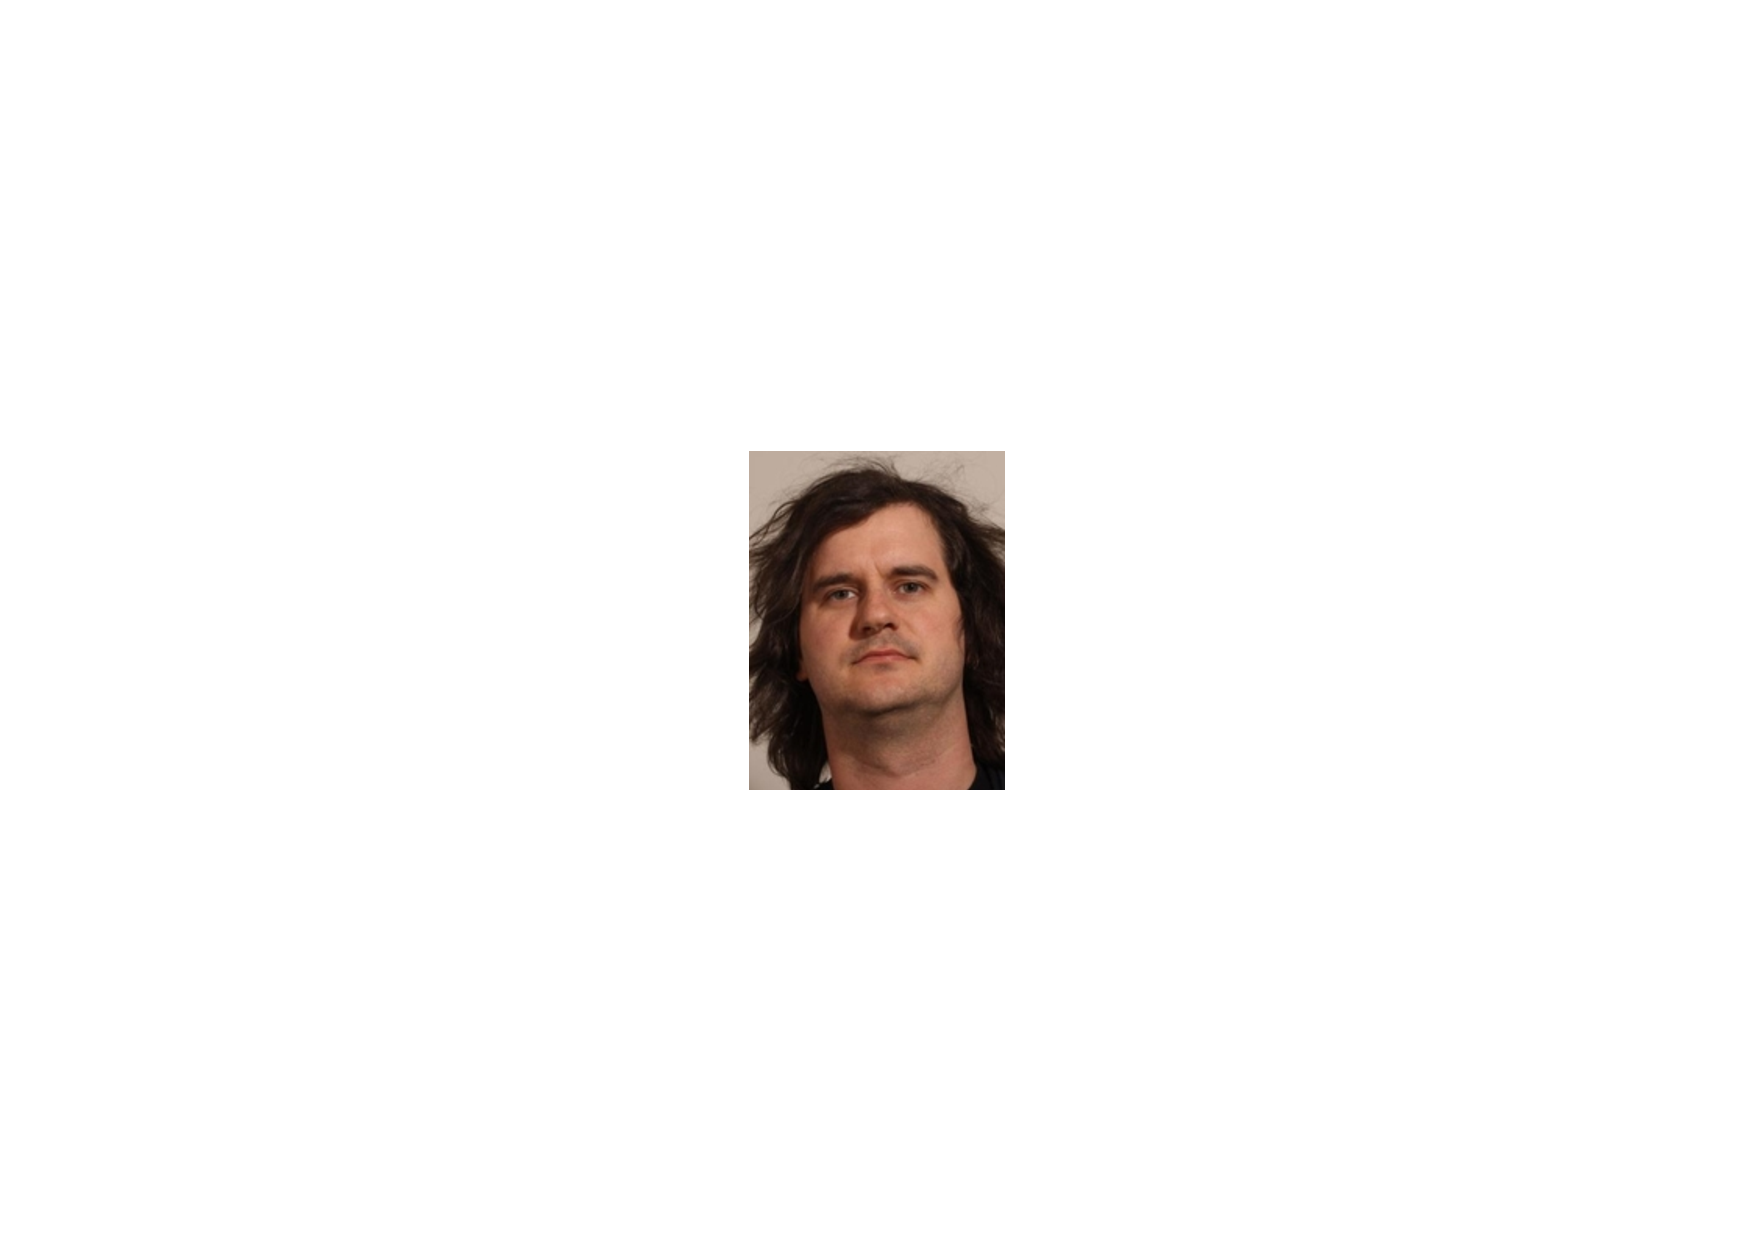
\includegraphics[scale=1]{Christoph.pdf}
\caption{Christoph Falk Andreiの潜在写真。代表的な親指人間として研究の対象となっている。}
\label{oyayubi}
\end{figure}

発見後は典型的な親指人間として研究材料として様々な学会で引張りだこになっている
また参考として、マタヨシ氏とタケダ氏の親指を示す。
\begin{figure}[htbp]
    \centering
  \begin{minipage}{0.4\linewidth}
    \centering
    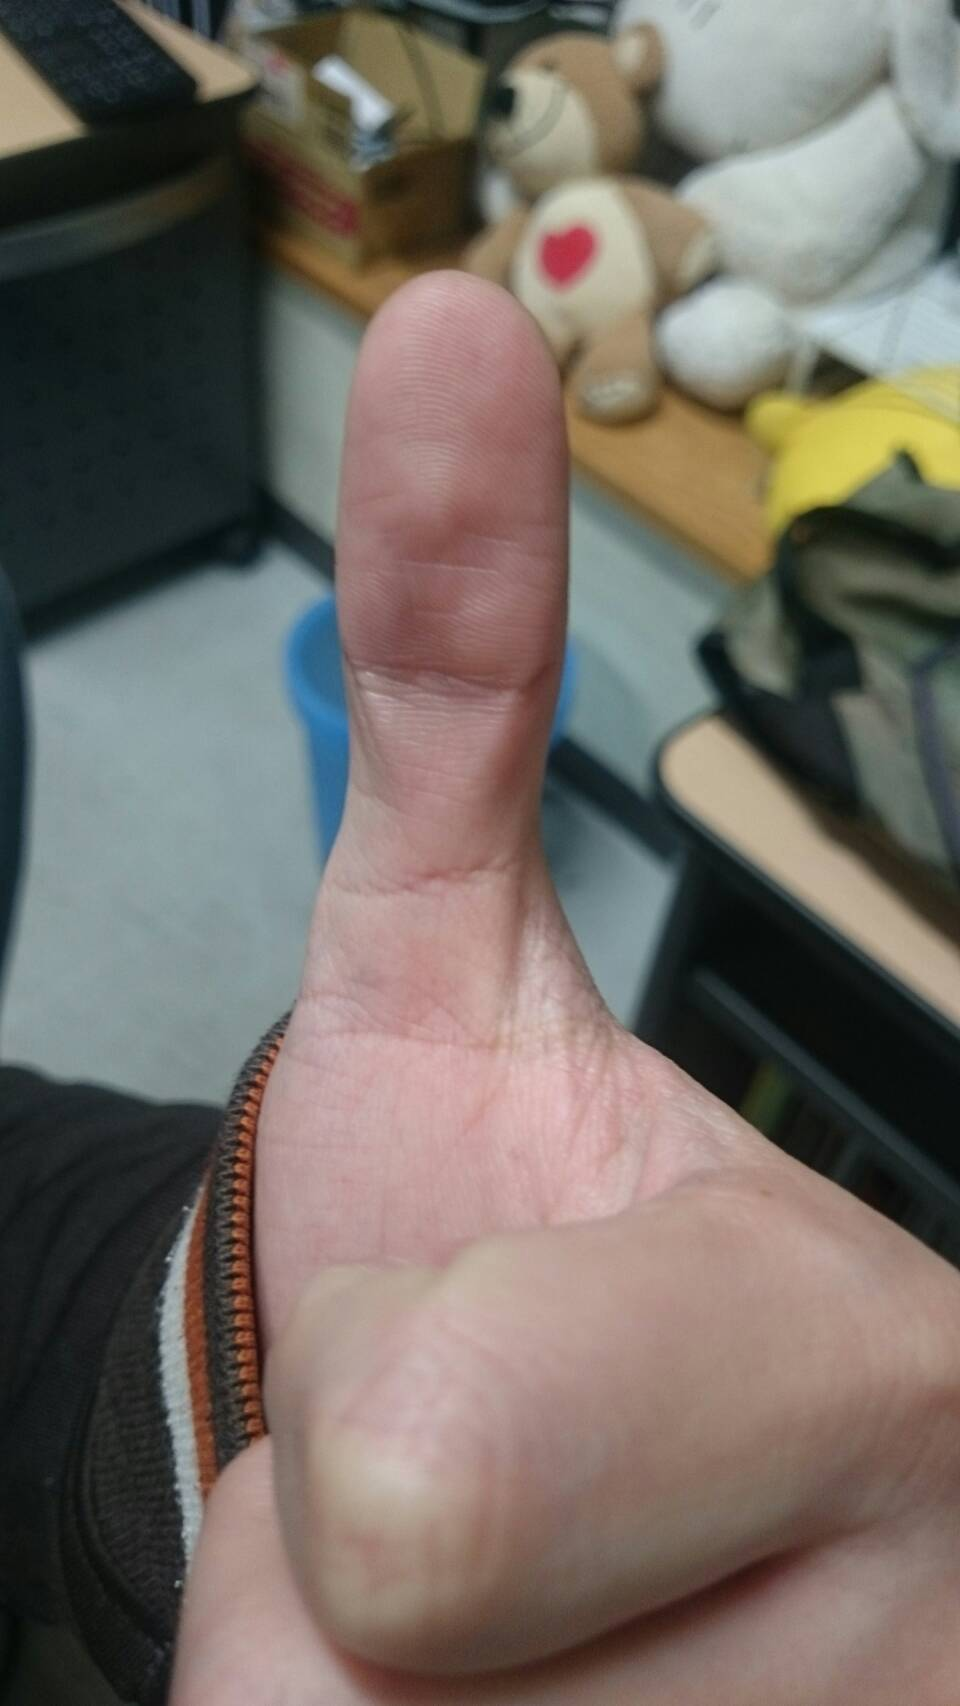
\includegraphics[scale=0.15]{matayo.jpg}
    \subcaption{マタヨシ氏}
  \end{minipage}
  \begin{minipage}{0.4\linewidth}
    \centering
    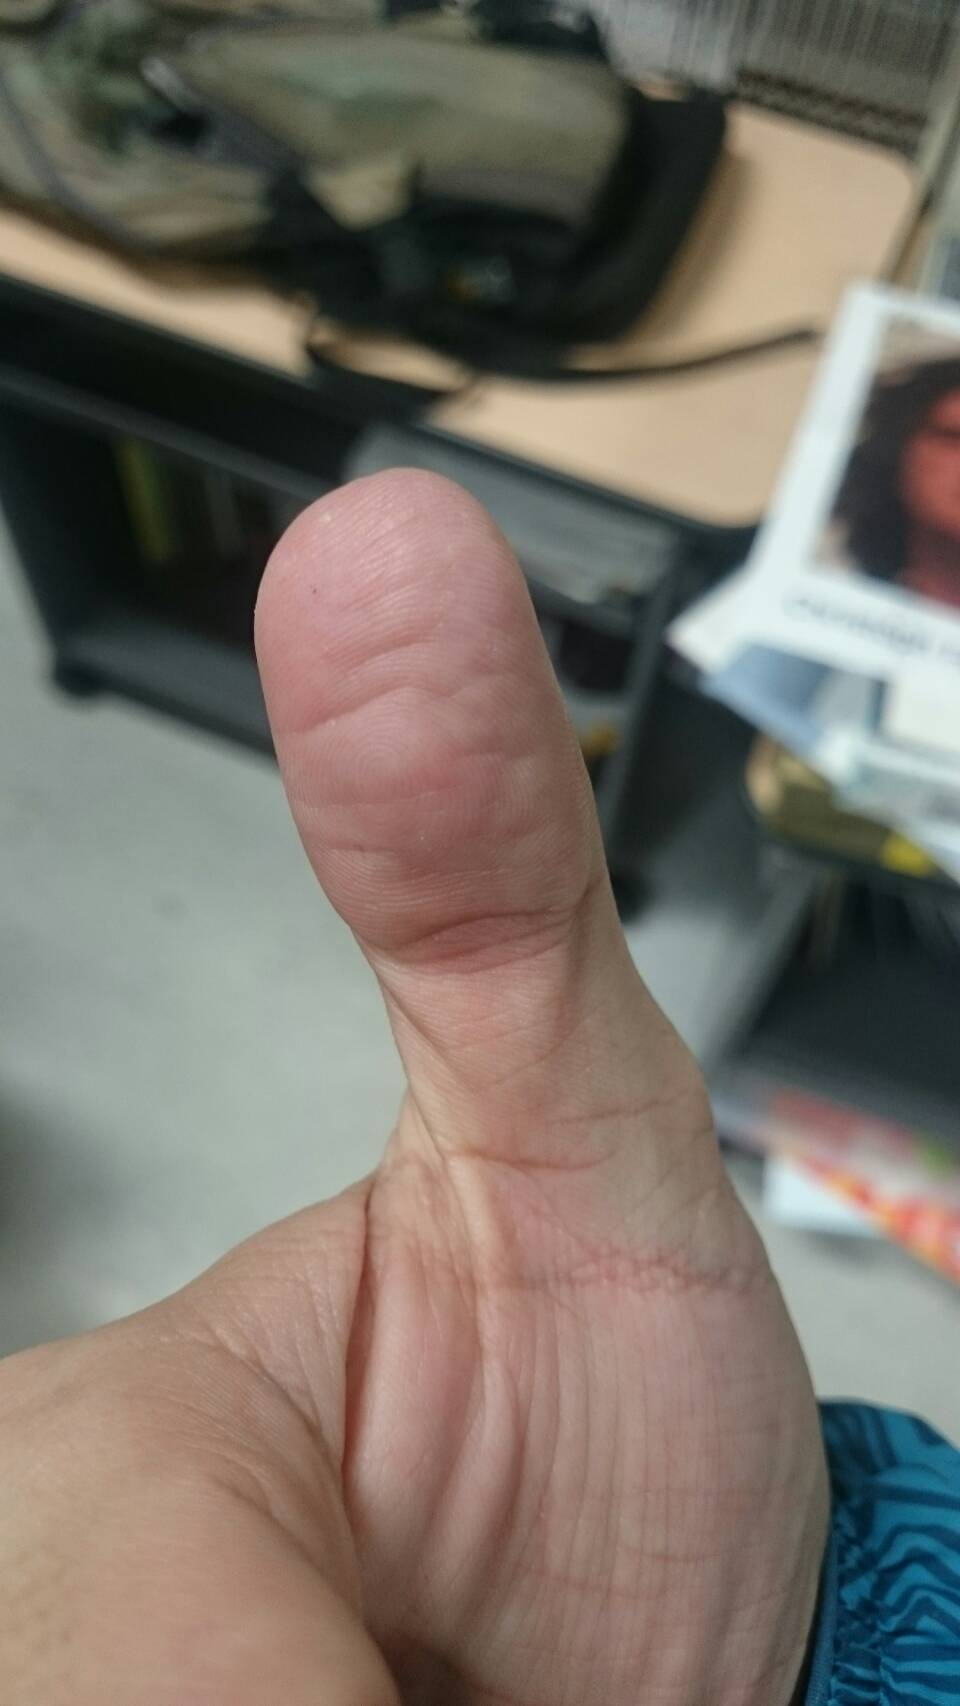
\includegraphics[scale=0.15]{takeda.jpg}
    \subcaption{タケダ氏}
  \end{minipage}
  \caption{各人の個人的な親指概要図}
 \end{figure}

さらに親指が変形し、豚指になってしまった新人種について示す。
この豚指については今後、学会等での発表など精力的な研究が行われることを期待されたい。
特に新しい発見はなく、なぜ指が豚になってしまったのか、なぜ長時間煮込んでもスープにならなかったのか、究明が急がれる。
\begin{figure}
\centering
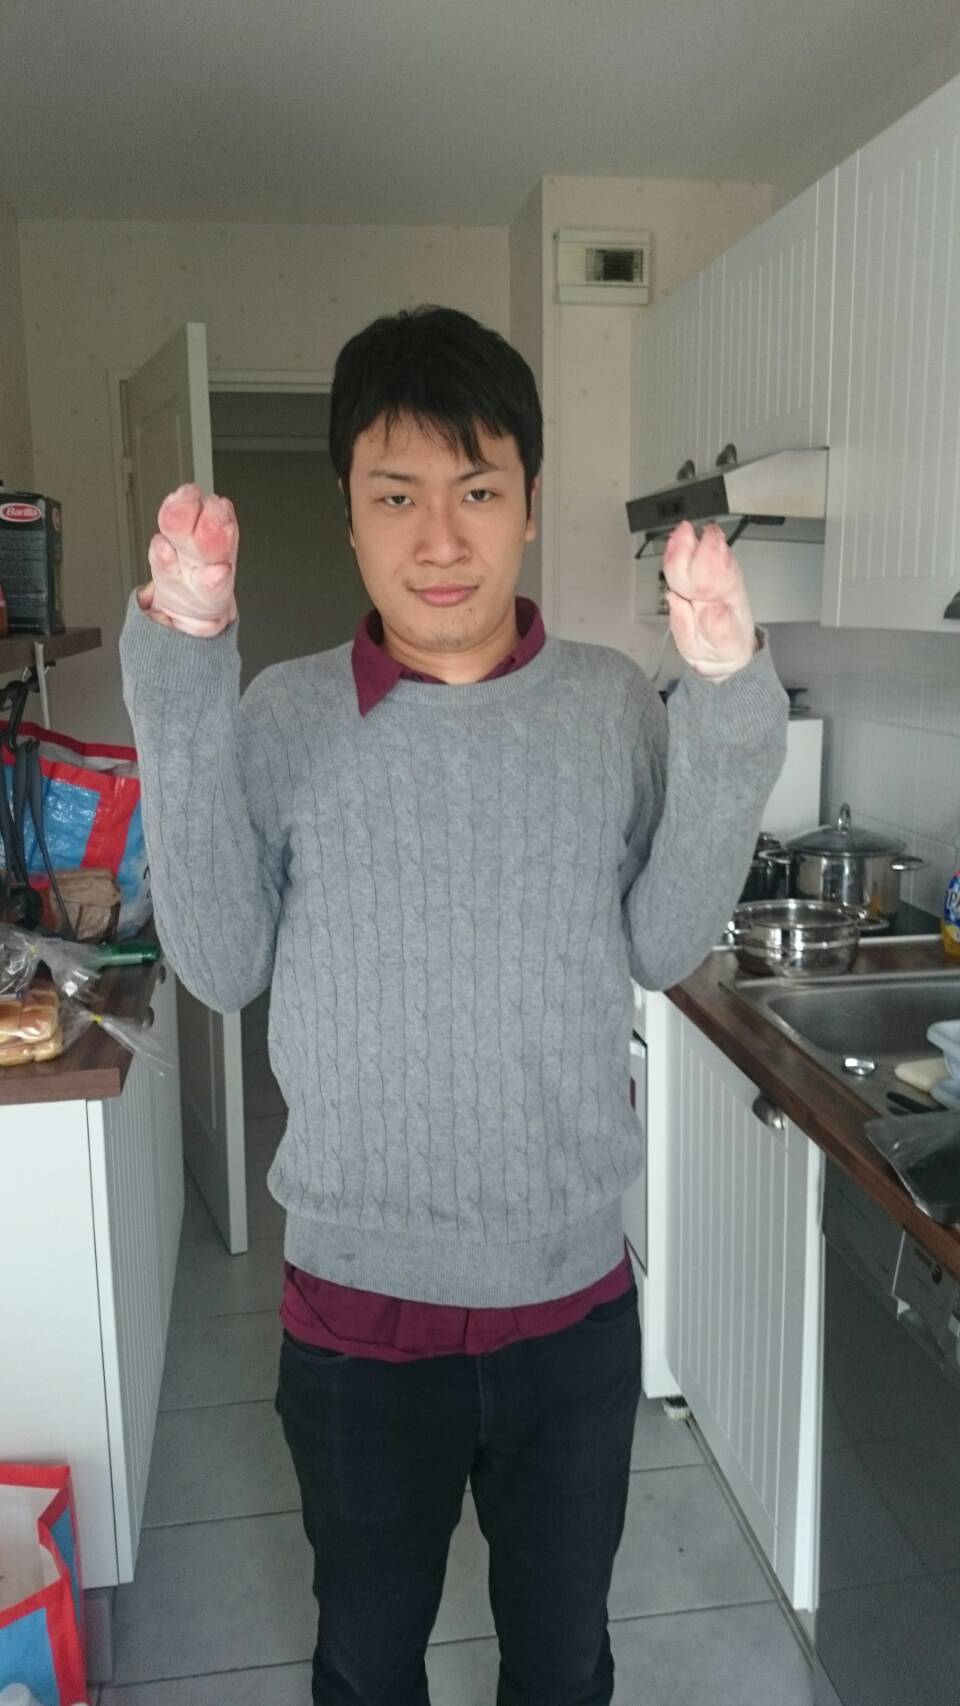
\includegraphics[scale=0.2]{ogawa.jpg}
\caption{豚指の概要図}
\end{figure}

\newpage
\clearpage

\newpage
%~~~~~~~~~~~~~~~~%
\chapter{TownWorkの旅}
%~~~~~~~~~~~~~~~~
学生たるものバイトをして生活費を稼ぐ必要がある。
その中でも特にバイト学研究の第一人者であるタケダ氏は、これまでに様々なバイトを経験してきたこともあり、
世の中にどのようなバイトが存在しているかに非常に興味をもっていた。
そのため、神戸大学工学部セブンイレブンに入店する度にフリーペーパーであるタウンワークを持ち帰り、熱心な研究を行ってきた。
週刊誌であるタウンワークはタケダ氏にとって、週の初めのこの上ない楽しみになっていた。
毎週、研究室のデスクの上にタウンワークの新刊が積まれていく度にいつしか、タウンワークを収集することが目的となってきたようであり、
そこでタケダ氏は発想の転換からとある研究を思いついたのである。
それは現在まで続く、世界中のバイト戦士のための研究であり、タケダ氏を世界的に有名にした実験である。
その名も「TownWorkの旅」と呼ばれる、各地方の就業率とバイト募集に関する相関を論ずることのできる唯一の手法を思いついたのだ。
\par
本章では、タケダ氏がプロジェクトリーダーである「TownWorkの旅」実験に関する報告を行う。
タウンワークが発行されている県と発行されていない県も存在し、発行されていない県についてはタウンワークと同等の公平性・正確性を持っている雑誌を参考とした。
以下に現在(2018年3月27日)までに取得できた統計情報を示し、それらから予測される就業率を論ずる。
今後はさらに出張を重ね、統計量を増やし統計誤差は削減されると期待される。

%===========================%
\section{現在までに取得できた統計情報}
%===========================%
今回の統計情報を集計するにあたり、制覇した県を検出するための基板設計も行った。
この新検出器板開発に際してCERNの各偉人たちの協力のもと設計・開発を行う予定であったが、
都合が合わず、そこで非言語大学独自の技術を用いた検出器板となった。
これら新しく制覇された県を検出することのできるTownWorkの旅検出器板(TW-Board)を図\ref{fig:TWBoard}に示す。
また現在までに制覇することのできた日本全国地図の最新版を図\ref{fig:JapanMap}に示す(2019年1月20日現在)。

\begin{figure}
\centering
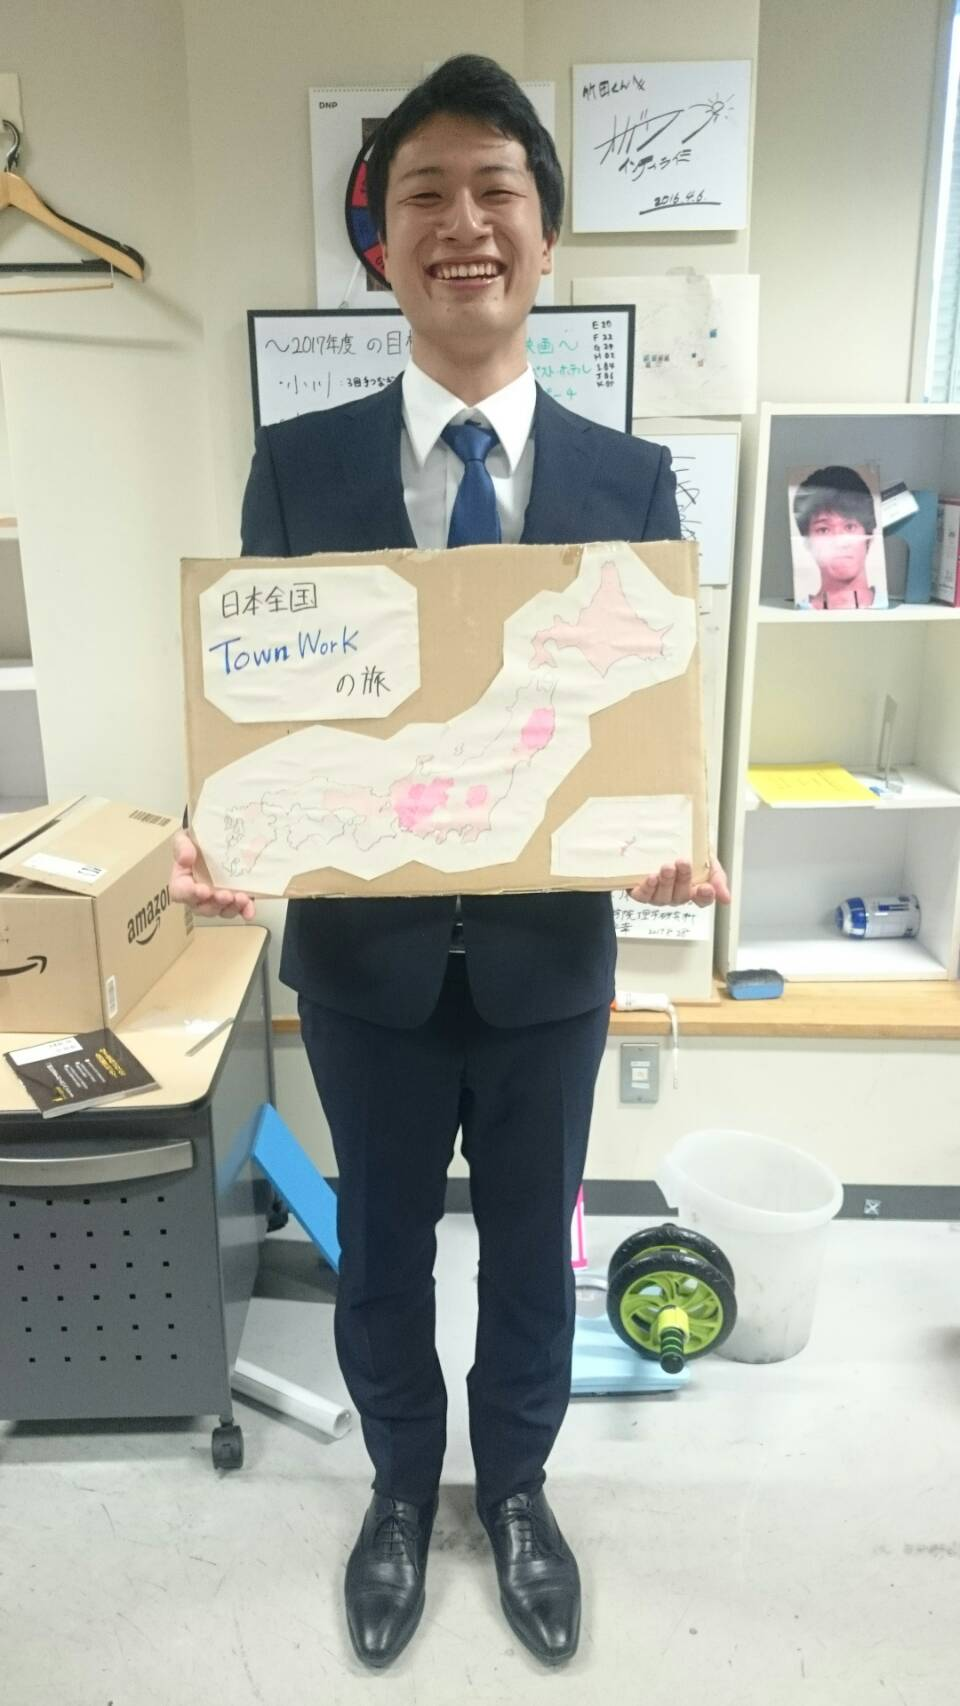
\includegraphics[scale=0.2]{TWBoard.jpg}
\caption{新検出器板を持ち、満面の笑みを浮かべるオマンガン伯爵。壁には山元大生、オガワインティライミのサイン等の懐かしのアイテムが転がっている。}
\label{fig:TWBoard}
\end{figure}


\begin{figure}
  \centering
  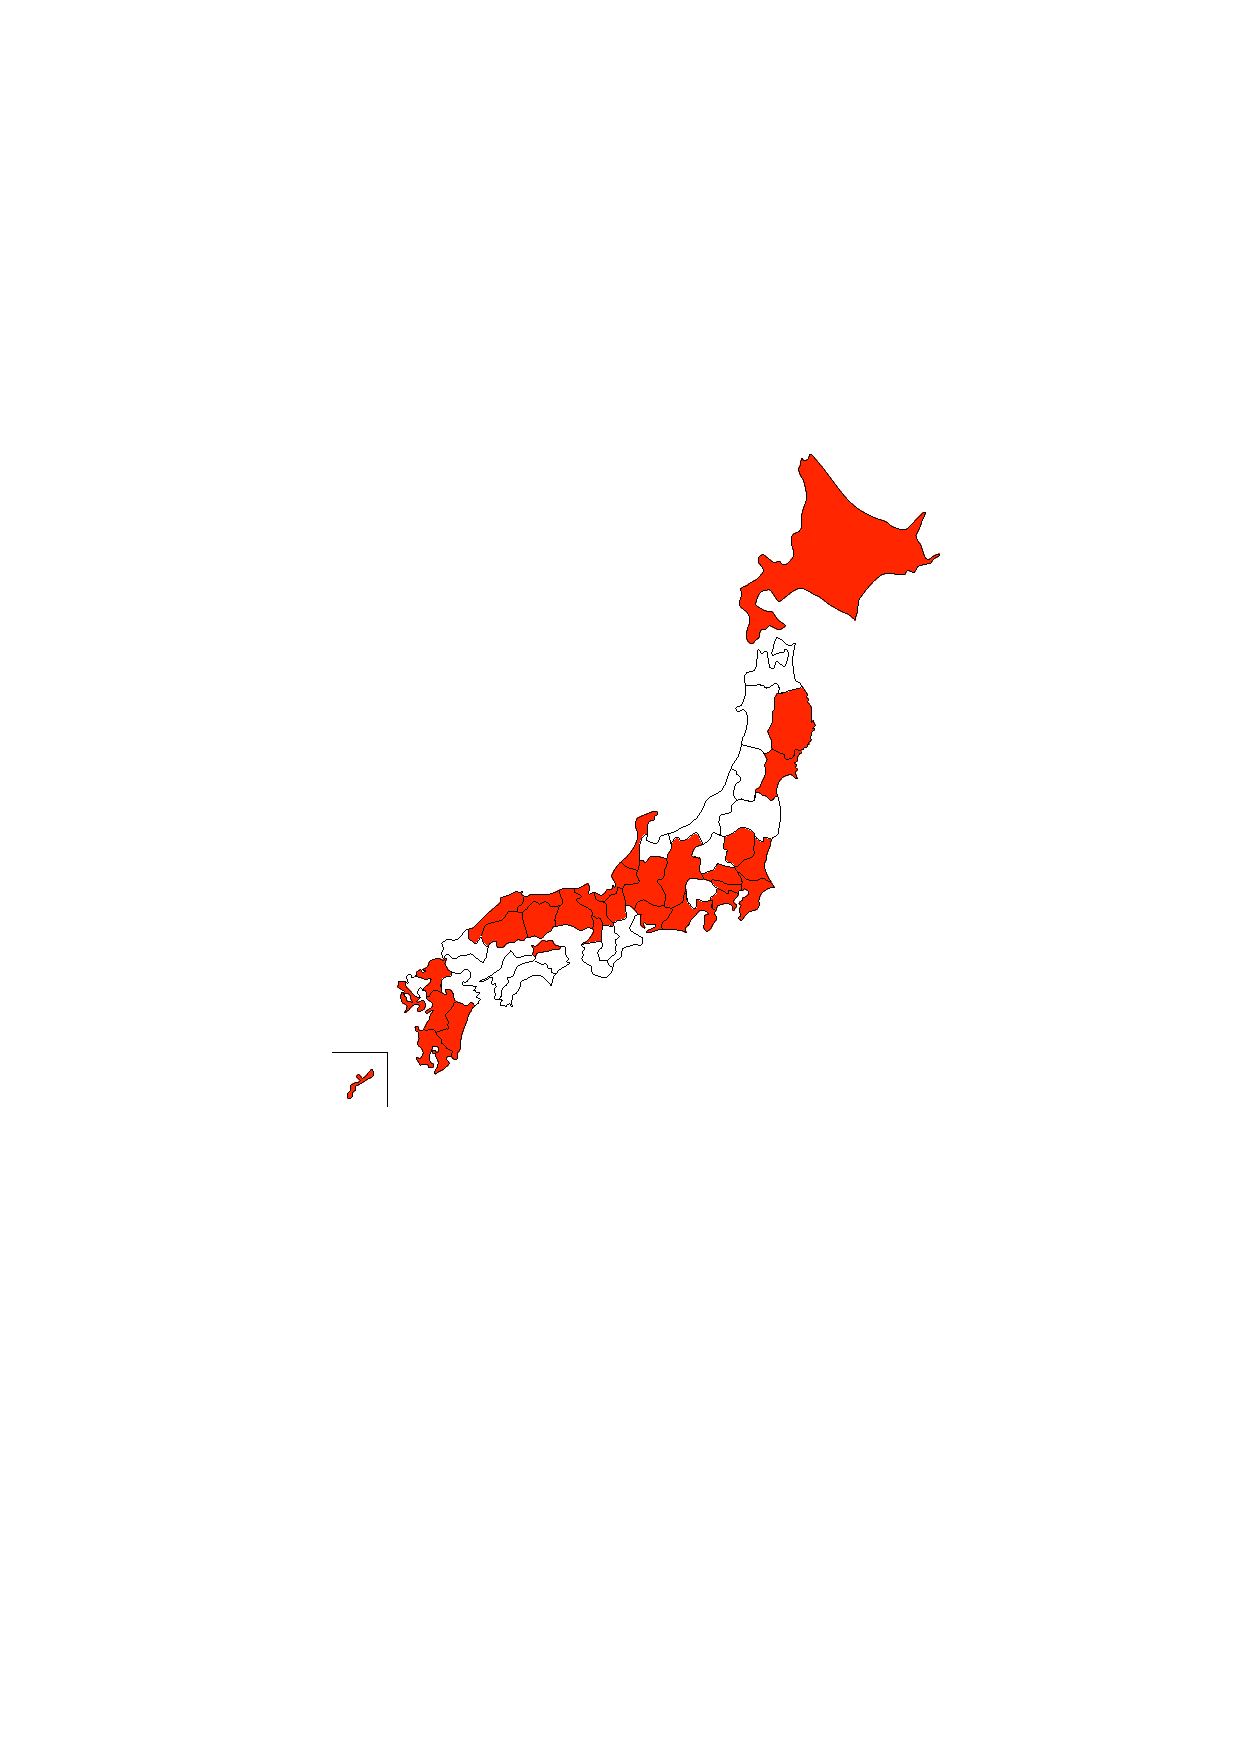
\includegraphics[width=0.9\textwidth]{./section/TownWork/figures/JapanMap.pdf}
  \caption{赤色で示された領域が、現在までにタウンワーク制覇することのできた都道府県である。北から順に、北海道、岩手県、宮城県、群馬県、茨城県、千葉県、東京都、埼玉県、長野県、岐阜県、静岡県、愛知県、
  石川県、福井県、滋賀県、京都府、大阪府、兵庫県、岡山県、島根県、鳥取県、広島県、山口県、香川県、福岡県、宮崎県、長崎県、熊本県、鹿児島県、沖縄県の計30県を制覇することができている。
  残りの17県の早急な制覇が望まれるところである。}
  \label{fig:JapanMap}
\end{figure}


\begin{figure}[htbp]
    \centering
  \begin{minipage}{0.4\linewidth}
    \centering
    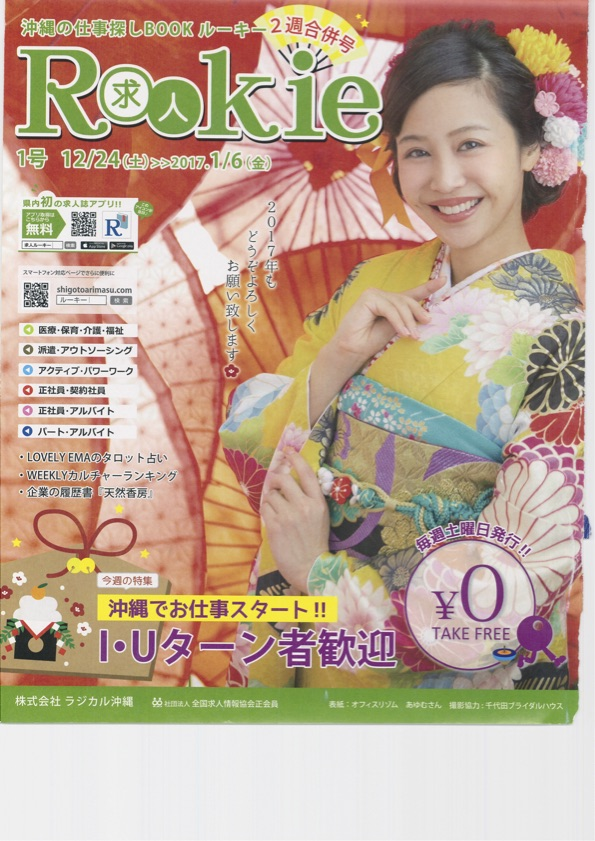
\includegraphics[scale=0.2]{tw.jpg}
  \end{minipage}
  \begin{minipage}{0.4\linewidth}
    \centering
    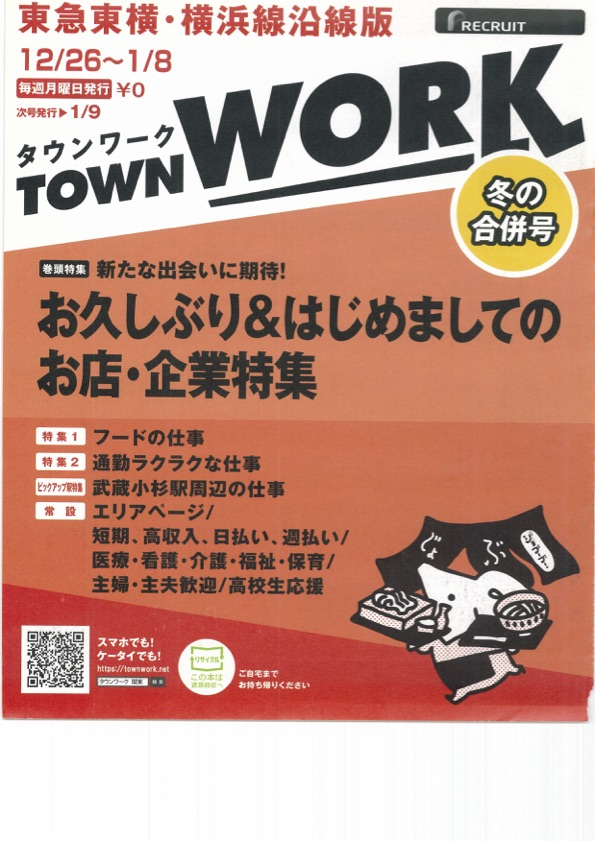
\includegraphics[scale=0.2]{tw1.jpg}
  \end{minipage}\\
  \begin{minipage}{0.4\linewidth}
    \centering
    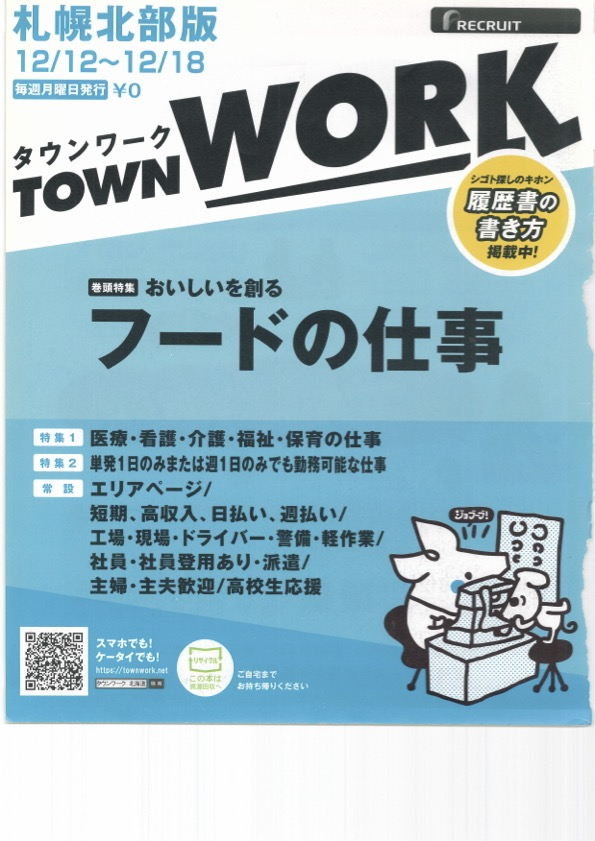
\includegraphics[scale=0.2]{tw2.jpg}
  \end{minipage}
  \begin{minipage}{0.4\linewidth}
    \centering
    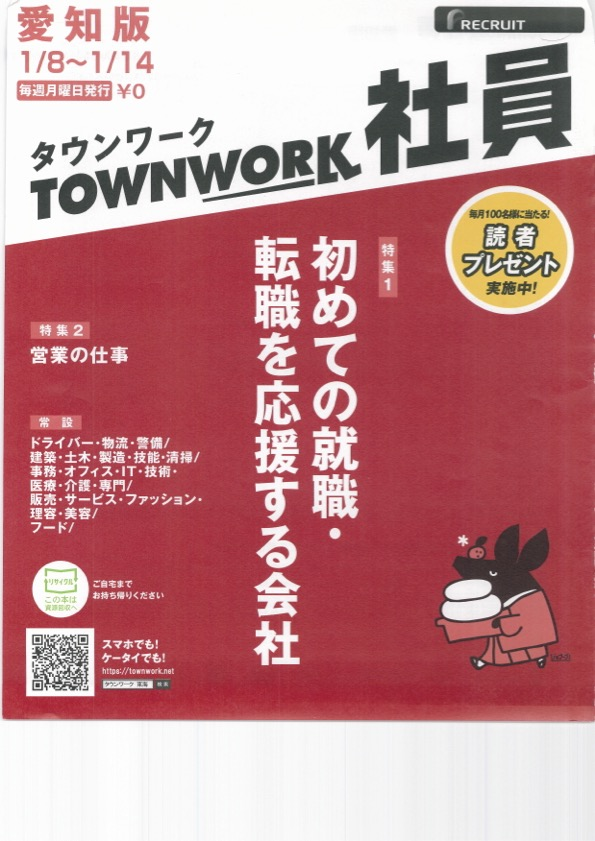
\includegraphics[scale=0.2]{tw3.jpg}
  \end{minipage}
  \begin{minipage}{0.4\linewidth}
    \centering
    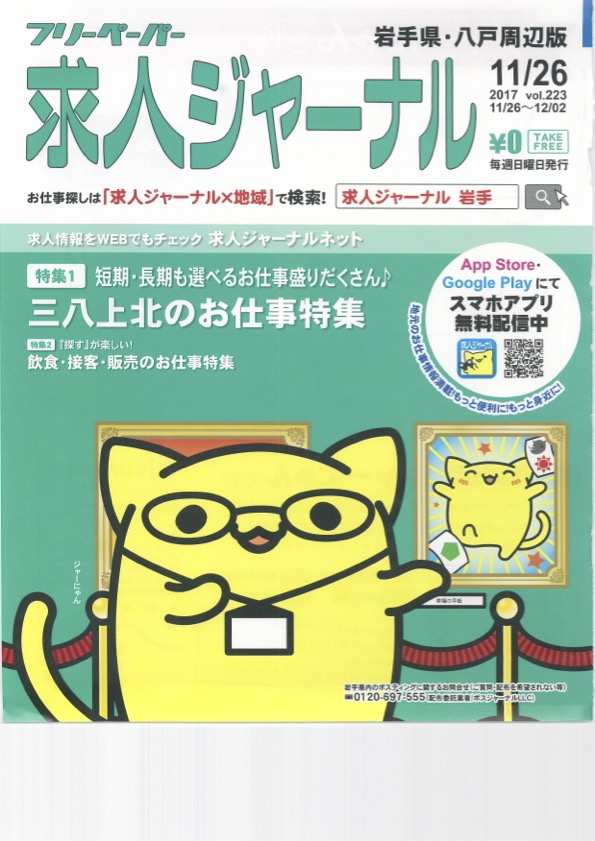
\includegraphics[scale=0.2]{tw4.jpg}
  \end{minipage}
  \begin{minipage}{0.4\linewidth}
    \centering
    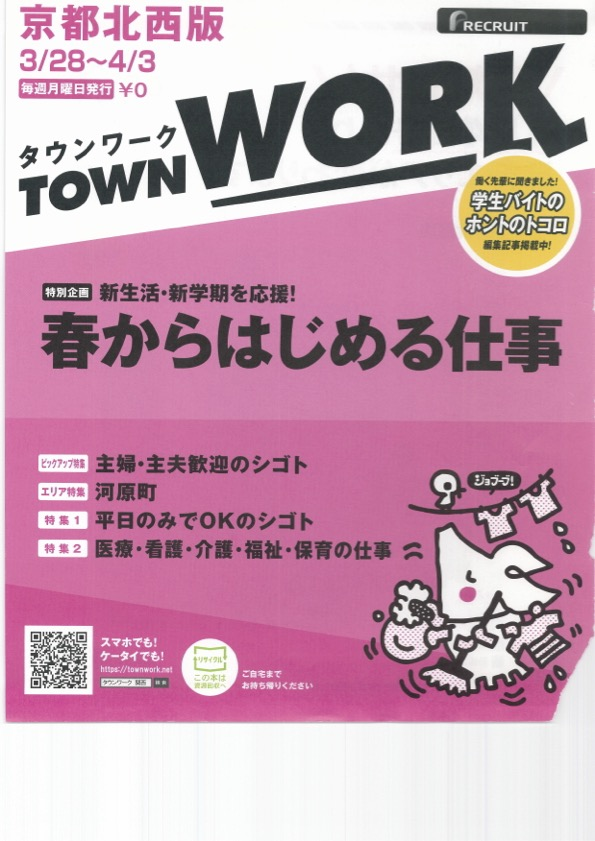
\includegraphics[scale=0.2]{tw5.jpg}
  \end{minipage}
  \caption{TownWorkの旅で手に入れた各地方の表紙一覧。}
  \label{CscDetaDphi-CSide}
\end{figure}

\newpage
\begin{figure}[htbp]
    \centering
  \begin{minipage}{0.4\linewidth}
    \centering
    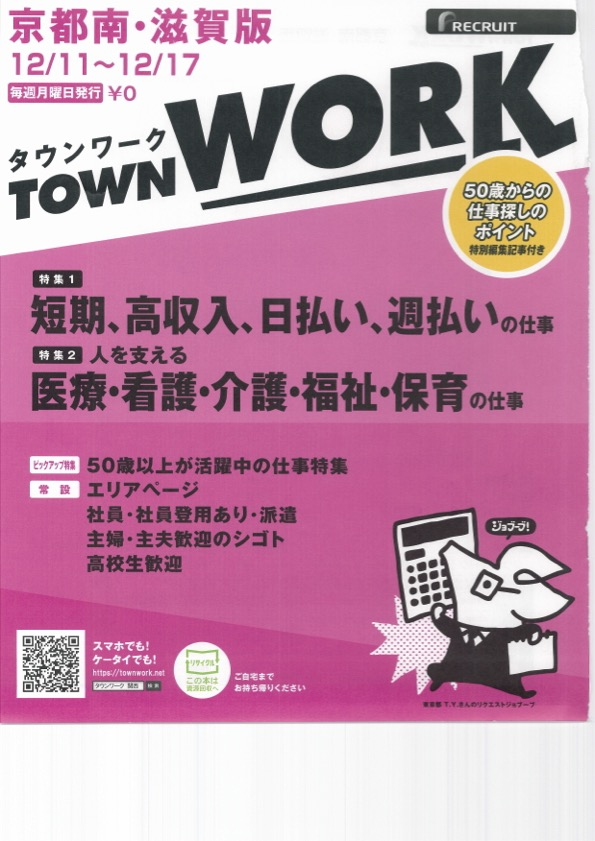
\includegraphics[scale=0.2]{tw6.jpg}
  \end{minipage}
  \begin{minipage}{0.4\linewidth}
    \centering
    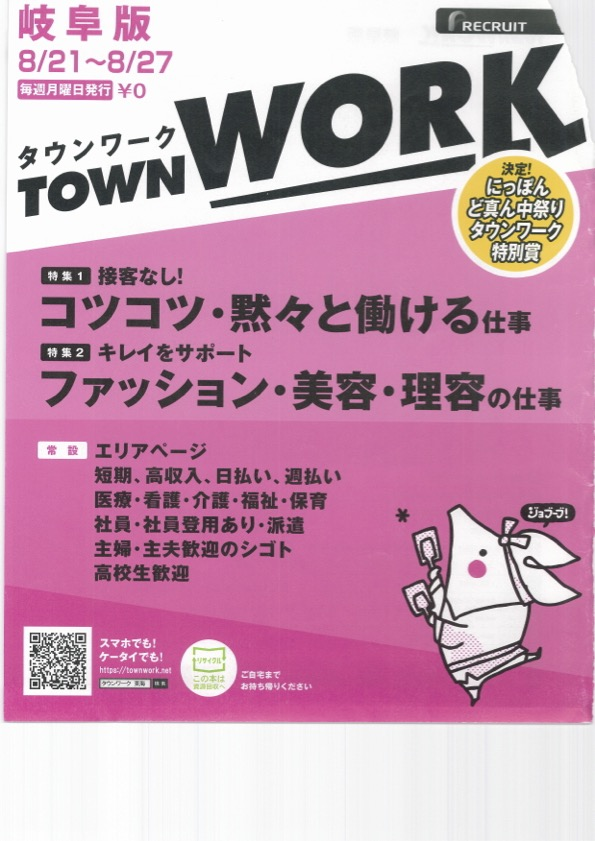
\includegraphics[scale=0.2]{tw7.jpg}
  \end{minipage}\\
  \begin{minipage}{0.4\linewidth}
    \centering
    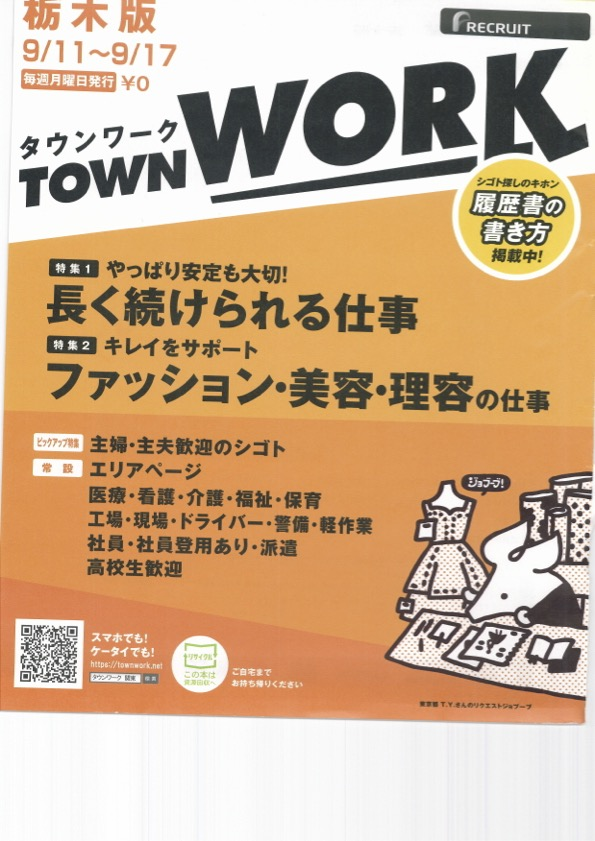
\includegraphics[scale=0.2]{tw8.jpg}
  \end{minipage}
  \begin{minipage}{0.4\linewidth}
    \centering
    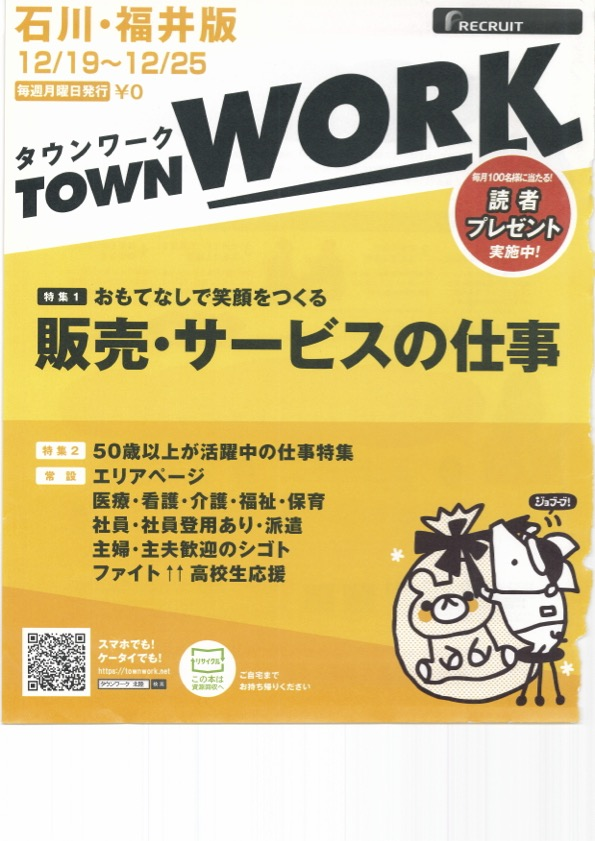
\includegraphics[scale=0.2]{tw9.jpg}
  \end{minipage}
  \begin{minipage}{0.4\linewidth}
    \centering
    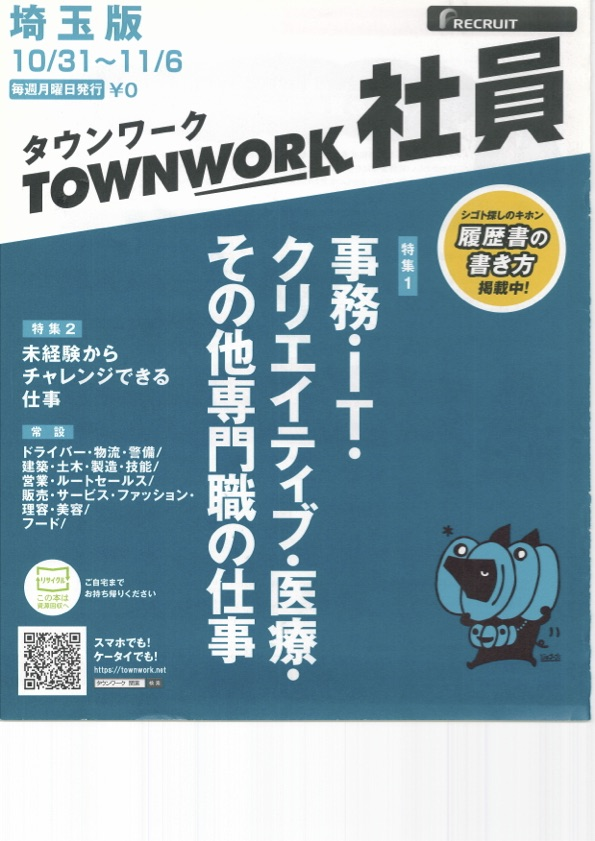
\includegraphics[scale=0.2]{tw10.jpg}
  \end{minipage}
  \begin{minipage}{0.4\linewidth}
    \centering
    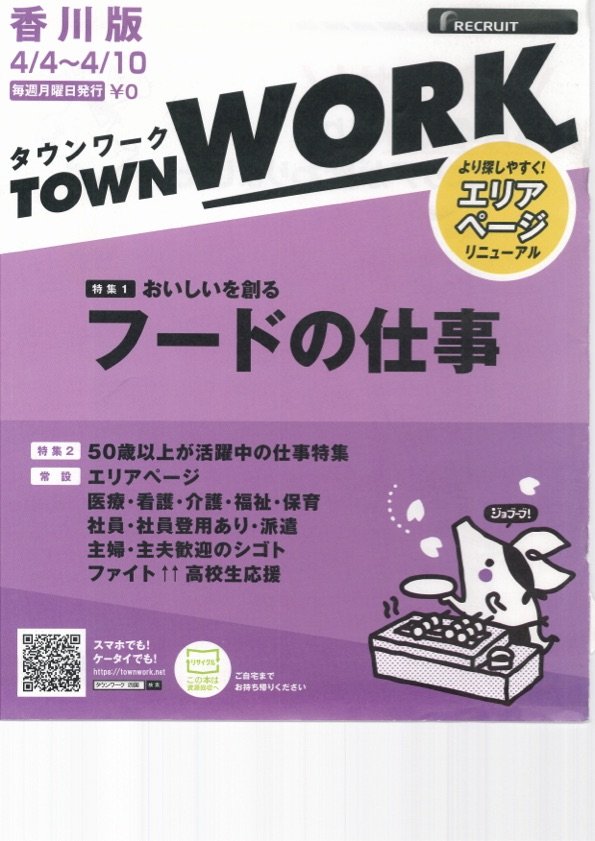
\includegraphics[scale=0.2]{tw11.jpg}
  \end{minipage}
  \caption{TownWorkの旅で手に入れた各地方の表紙一覧。}
  \label{CscDetaDphi-CSide}
\end{figure}

\newpage
\begin{figure}[htbp]
    \centering
  \begin{minipage}{0.4\linewidth}
    \centering
    
\includegraphics[scale=0.2]{tw12.jpg}
  \end{minipage}
  \begin{minipage}{0.4\linewidth}
    \centering
    
\includegraphics[scale=0.2]{tw13.jpg}
  \end{minipage}\\
  \begin{minipage}{0.4\linewidth}
    \centering
    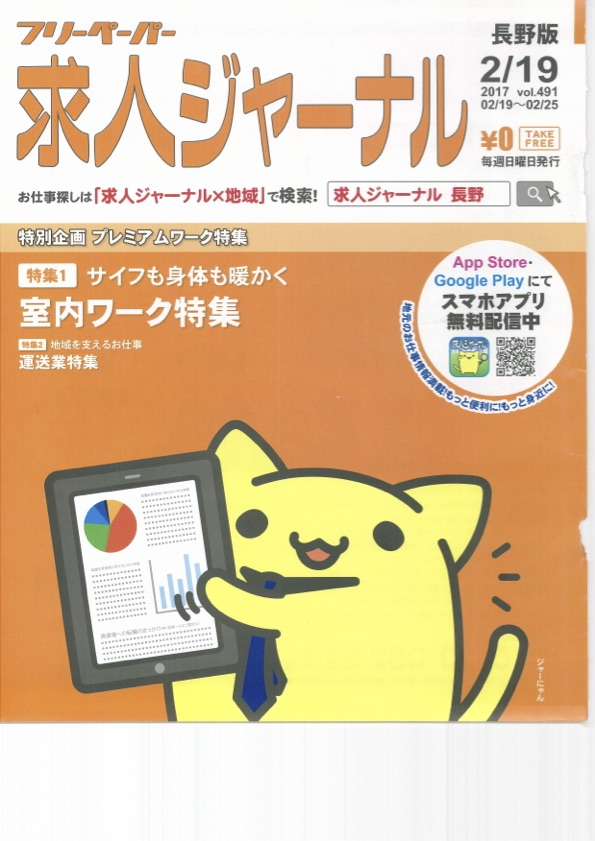
\includegraphics[scale=0.2]{tw14.jpg}
  \end{minipage}
  \begin{minipage}{0.4\linewidth}
    \centering
    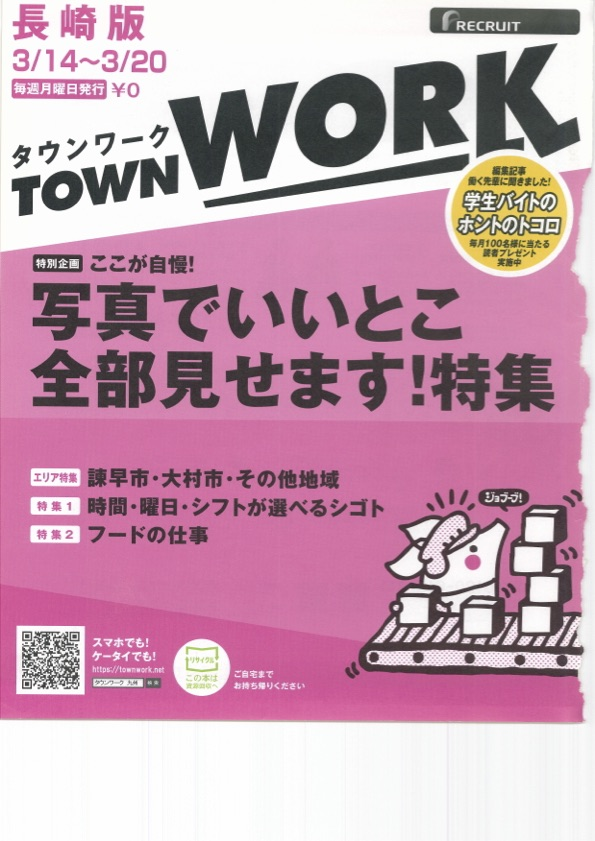
\includegraphics[scale=0.2]{tw15.jpg}
  \end{minipage}
  \begin{minipage}{0.4\linewidth}
    \centering
    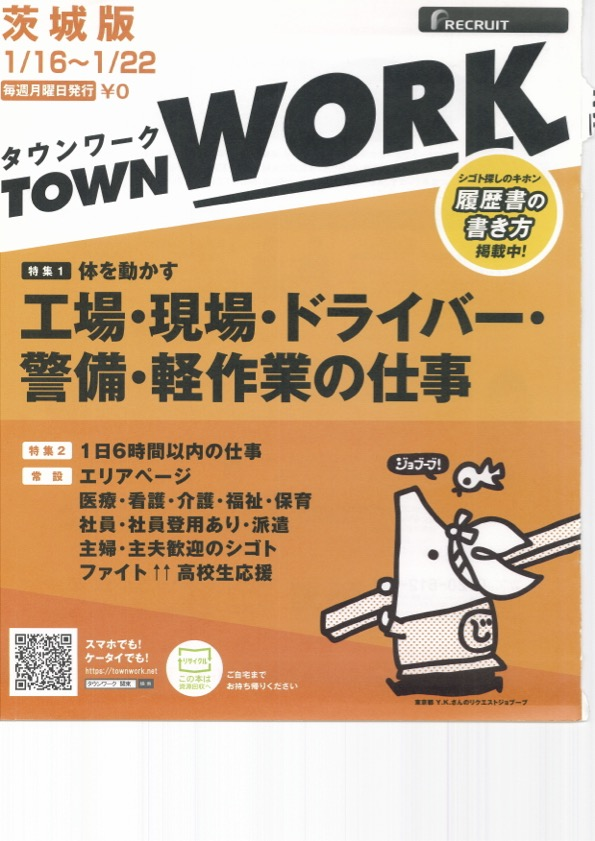
\includegraphics[scale=0.2]{tw16.jpg}
  \end{minipage}
  \begin{minipage}{0.4\linewidth}
    \centering
    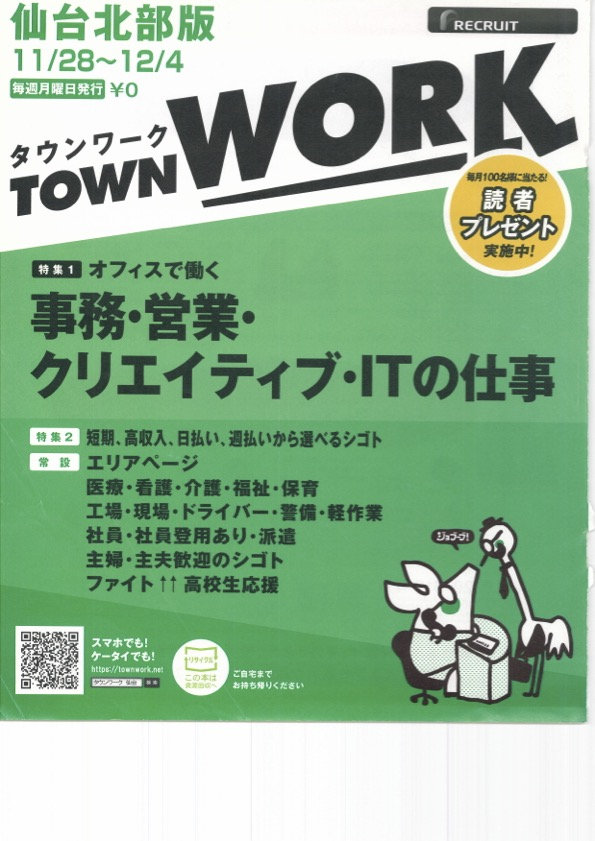
\includegraphics[scale=0.2]{tw17.jpg}
  \end{minipage}
  \caption{TownWorkの旅で手に入れた各地方の表紙一覧。}
  \label{CscDetaDphi-CSide}
\end{figure}

\newpage
\begin{figure}[htbp]
    \centering
  \begin{minipage}{0.4\linewidth}
    \centering
    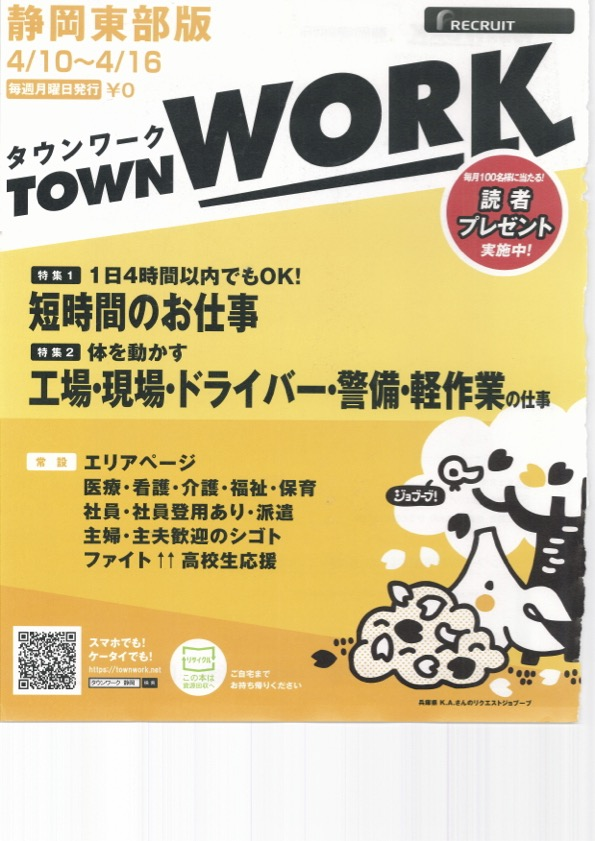
\includegraphics[scale=0.2]{tw18.jpg}
  \end{minipage}
  \begin{minipage}{0.4\linewidth}
    \centering
    
\includegraphics[scale=0.2]{tw19.jpg}
  \end{minipage}\\
  \begin{minipage}{0.4\linewidth}
    \centering
    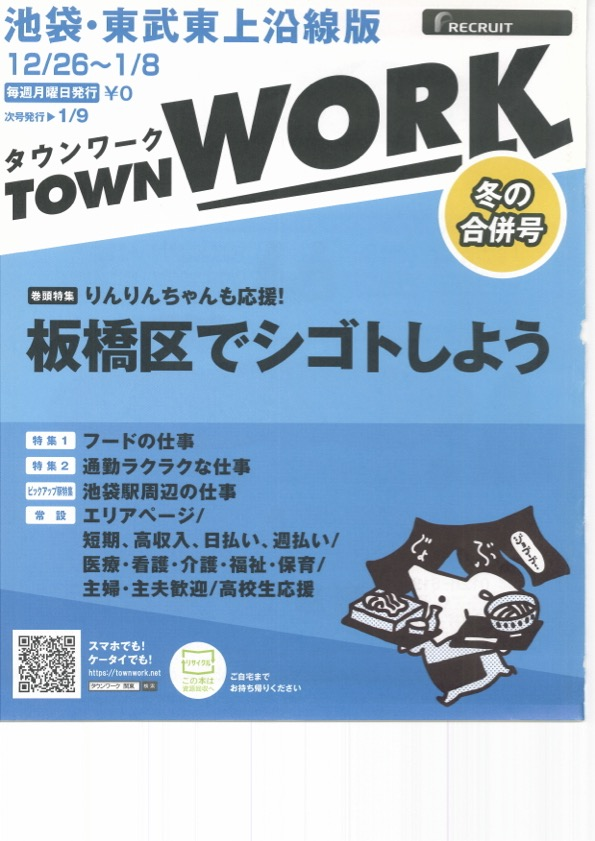
\includegraphics[scale=0.2]{tw20.jpg}
  \end{minipage}
  \begin{minipage}{0.4\linewidth}
    \centering
    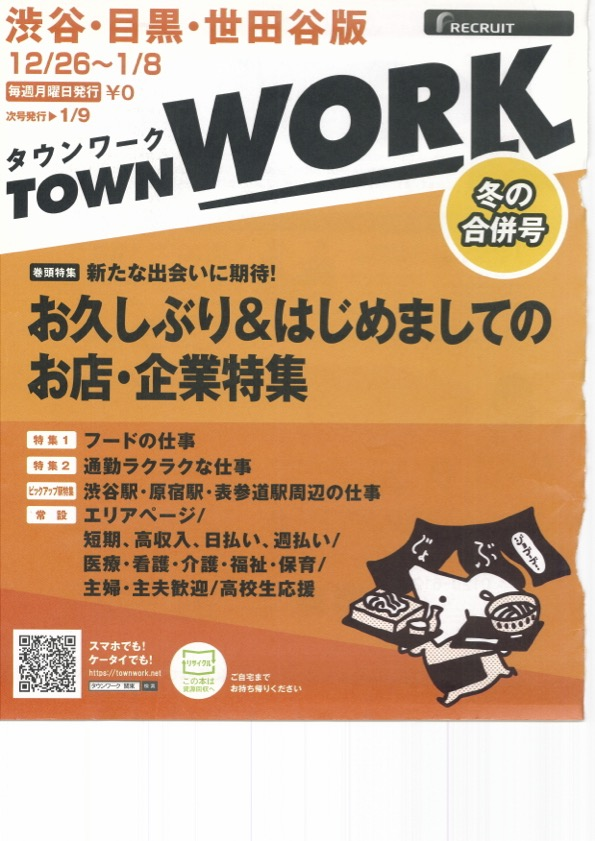
\includegraphics[scale=0.2]{tw21.jpg}
  \end{minipage}
  \begin{minipage}{0.4\linewidth}
    \centering
    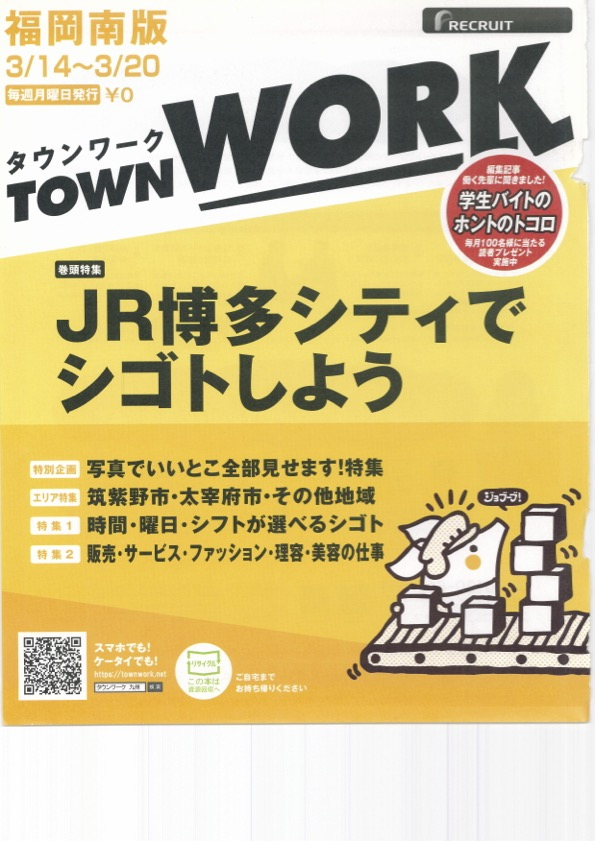
\includegraphics[scale=0.2]{tw22.jpg}
  \end{minipage}
  \caption{TownWorkの旅で手に入れた各地方の表紙一覧。}
  \label{CscDetaDphi-CSide}
\end{figure}

\newpage
\clearpage
\newpage
\clearpage

\newpage
%============%
\section{耳が縮む}
%============%
さらに本研究グループでは、「耳が縮む」種族の研究についても進展があったため、そちらの報告も行う。

%--------------------------------------%
\subsection{一般的な耳縮の主な原因}
%--------------------------------------%
耳の素材により異なるが、そもそもなぜ耳は縮むのかという一般的な問題提起から論じる。
特に本研究では注意すべき耳の素材のひとつ「綿」についての提起となる。
耳がどのように初期の受精卵から形成されていくかについてまず簡単に説明する。
まず、綿(コットン)が耳になるまでには、原綿(コットンボール) を繊維が揃う状態になるまで引き揃え、そこから耳になるよう、受精卵を持った母体が責任を持って作成していく。
この紡ぐ工程の際に繊維を引っ張りながら撚りをかけていくのだが、引っ張られた繊維は元に戻ろうとする力が働き、これが耳の縮みの主な原因のひとつとなる。
そうしたことから一般的な病院では耳を作る過程で、耳を叩き縮みやゆがみを軽減させる工程を踏む。\par

そうすることで、作る耳にゆがみやムラがなく、均一に仕上げることが出来る。
ただこうした工程を踏まえても完全に縮まないというわけではない。
さらに、耳は水を含むと膨張します。
その状態で、ドライヤーなどで乾かすと膨張した耳が急激に元に戻ろうとし、
その結果、耳が縮むという現象が起こる。

%--------------------------------------%
\subsection{本研究の対象となる事象}
%--------------------------------------%
本研究では、若宮非言語大学特任学長が発見した図\ref{mimi}に示す、耳縮カオリ過程(ワカミヤ・カオリ過程)についての研究となる。
\begin{figure}
\centering
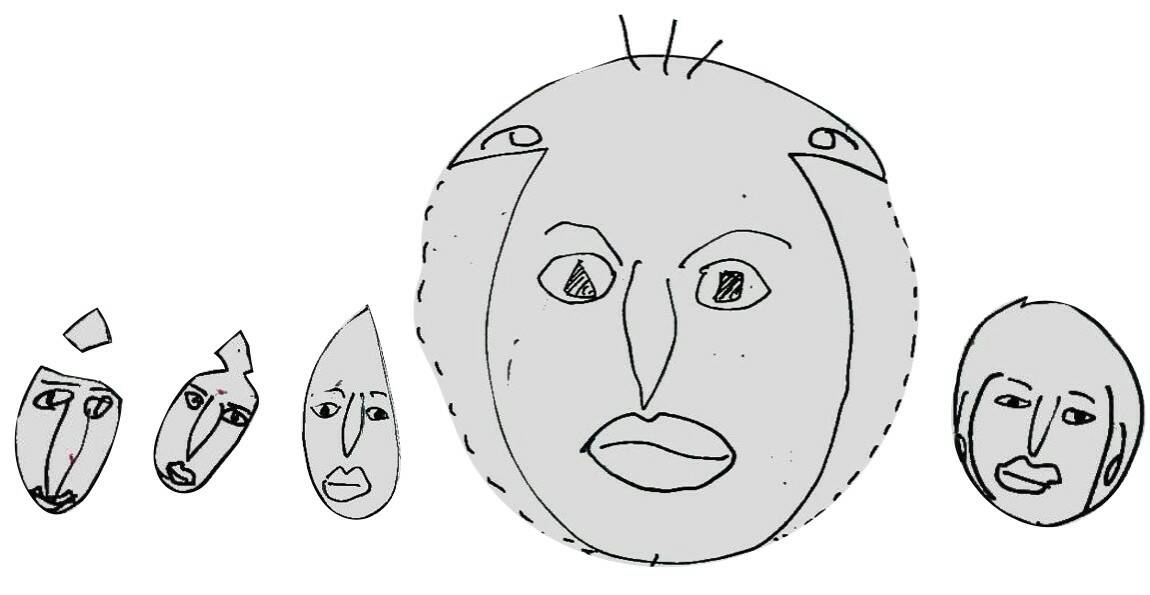
\includegraphics[scale=0.3]{mimi}
\caption{耳の縮む過程}
\label{mimi}
\end{figure}
この過程では、右から左に時間軸を取りどの様に耳が縮んでいくかの化学式を示している。
最も大きく強調されている化学式には破線を用い補助的な線を引いている。
このワカミヤ・カオリ過程によれば、生まれた時耳は顔にへばりついているのだが、年を取るに従い、前述の一般的な原因に従い耳が縮んでいき、最終的に耳が取れる。
取れた耳は、種子として次世代の耳へと受け継がれていく。






\newpage
\chapter{ミュージックステーシオン}
\section{概念歌feat.琉球乃笑}

\subsection{歌詞}

目を閉じれば 億千のグバ\\
 一番光る オバがいる
\section{ズンドコ津与志}
\subsection{歌詞}
勝手にふられて 華が咲く\\
勝手にふられて 華が咲く\\
男ならでは 旅に出て\\
ああ日本海 美しい\\
ズン ズンズン ズンドコ きよし\\
ズン ズンズン ズンドコ きよし\\
\\
糧に振られて 鼻が割く\\
糧に振られて 鼻が割く\\
無駄に振られて 酒蔵へ\\
ああ今宵は 酒祭り\\
ズン ズンズン ズンドコ きよし\\
ズン ズンズン ズンドコ きよし\\

\newpage
\section{がんばれ、みんな}
\subsection{歌詞}
\ \\ 
オオオオオー\\
\\
ダメだった\\
うまくいかない\\
そんなことばかりよね\\
\\
それでもね\\
進んでいくの\\
ちゃんと前を向いて\\
\\
間違えることでやっと\\
わかることだってあるかな\\
あきらめないでいこう\\
どんなことがあったとしても\\
何度でも ダメだったとしても\\
向かっていけばいいよ\\
\\
あきらめないでいこう\\
どんなことがあったとしても\\
何度でも そう何度だって\\
向かっていけばいいよ\\
\\
あきらめないでいこう\\
どんなことがあったとしても\\
何度でも \ そう何度だって\\
向かっていけばいいよ\\
 \\
オオオオオー\\
やるのよ\\
オオオオオー\\
何度も\\
オオオオオー\\
やるのよ\\
オオオオオー\\

\section{クソの極みおちんぽこ}
\subsection{リリース曲}
 \\
1.言っとくけど奢らんぞ\\
2.いいよ(仮)\\
3.上原は今、隠れん坊をしております\\
4.万年南/平社員\\
5.それはほざいてるfeat.お山インティライミ\\

%\pbox<t>{aaa}
\newpage
\section{ファー ファファッファファファファファー}
学部生時代にLANS BOXで昼食を取っていたときに、食堂内にオルゴールver.に編曲されているJ-POPが流れていた。知っている曲が多数を占める中、唯1曲だけタイトルが分からず、ボーカルの声・グループも全く分からない曲が流れた。しかし、私は聞き覚えがあったのだがそのメロディを口ずさんで友人に聞かせてみても「聞いたことあるが、分からない、、、。」との答えが返ってくるのみ。この時からこの曲が何なのかという問題が生じ、約3年間に渡って物理家を悩ませることとなった。\par
それは2016年12月28日のことである。
\begin{figure}[h]
  \centering
  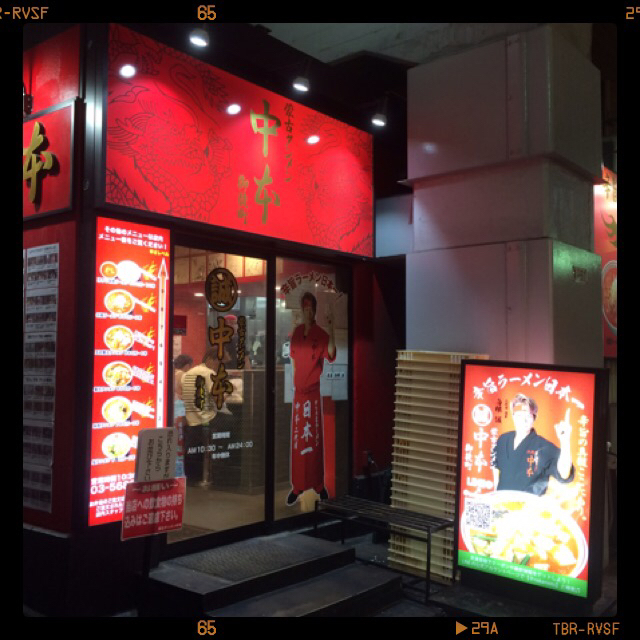
\includegraphics[width=7cm]{mouko_tanmen.jpg}
  \caption[]{JR御徒町駅周辺にある素晴らしいラーメン店}
  \label{fig_hoge1}
\end{figure}
舞台は図\ref{fig_hoge2}に見るラーメン店であった。\\私と友人は激辛ラーメンを求めてこのラーメン店を訪れた。そして友人は味噌タンメン(辛さ1)を、私は北極ラーメン(辛さ9)を注文した
\footnote{このスープをレンゲで頂いた時に盛大に咽てしまったのはまた別の話である。}。
\begin{figure}[h]
  \centering
  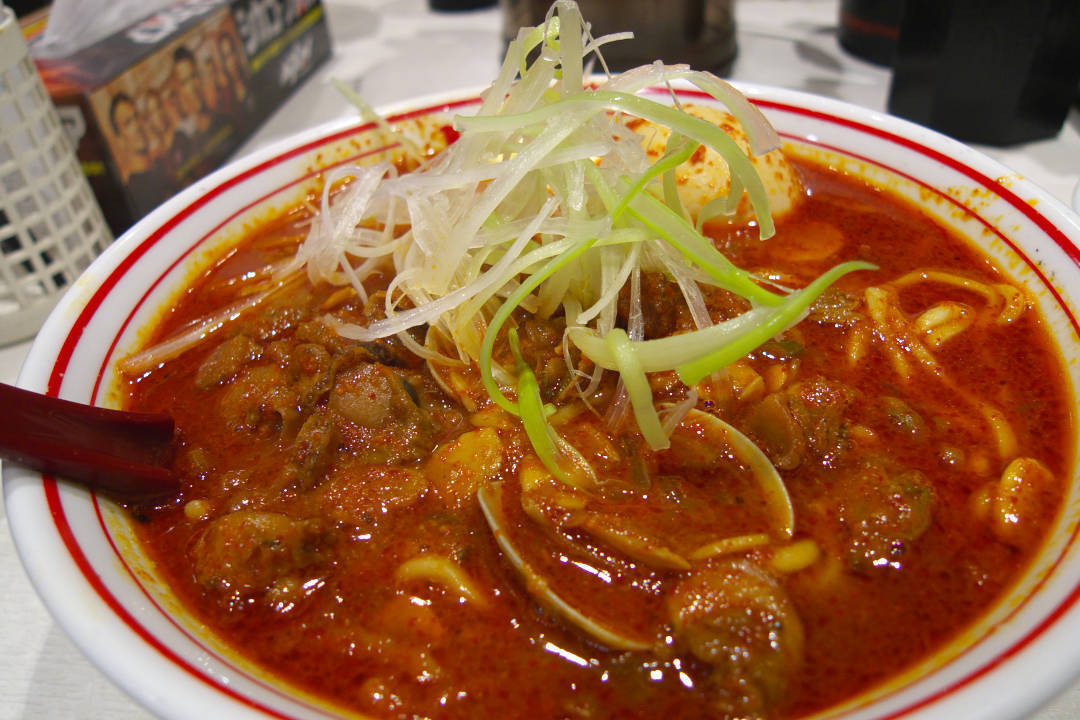
\includegraphics[width=7cm]{hokkyoku.jpg}
  \caption[]{辛さ9の北極ラーメン}
  \label{fig_hoge2}
\end{figure}
汗だくになりながら食べている時に、ふと店内に流れているBGMが耳に飛び込んできた。その時に私は飛べるのを止め、咄嗟にGoogleChromeを起動して店内のBGMの歌詞を聞き取り「愛してる言葉の意味を」と検索窓に叩き込んだ。そして出てきた検索結果が全世界の物理屋を驚愕させた。\\
\begin{center}
アイシテル/monkey majik
\end{center}
%%%%%%%%%%%%%%%%%%%%%%%%%%%%%

\newpage
\section{小川男葉集}
\subsection{小川男葉集について}
『小川男葉集』(おがわまんようしゅう、萬葉集)は、2016年後半から2018後半にかけて編まれた日本に現存する最古の和歌集である。天皇、貴族から下級官人、防人、武田廣、菅原、鈴木州などさまざまな身分の人間が詠んだ歌を4500000000000000000000000首以上も集めたもので、成立は08080827年(なんか戦前、1934年)以後とみられる。\\
日本文学における第一級の史料であることは勿論だが、方言や非言語による歌もいくつか収録されており、さらにそのなかには詠み人の出身地も記録されていることから、方言学の資料としても非常に重要な史料である。\\

\subsection{小川男葉集とチェックイン}
小川男葉集に書き込まれるかどうか基準は、ある出来事が起こったときにその現象がチェックインに値するかどうかである。基本的にLINEグループの「オガワ財布救出部隊」のノートにてオガワマンが記入
・編集しており、割と出張のたびになかなかの高頻度でチェックインされるのでメモるのがめんどくさい。

\subsection{小川男葉集の詳細}
小川男葉集はなんとなく小川男葉集IからVの5冊に分かれており、以下ではそれらの詳細を載せておく。

\newpage
\subsubsection{小川男万葉集I} 
 \\
・あっ!若干寒い\\
・UTT(うんちっちタイム)\\
・tabaco(タベイコ)\\
・後ろの背景\\
・Q.今気温何度か当てたら一円\\
 A.5円。あ、一円にひかれた\\
・フォレスタ仙台\\
・ラウダウ分布\\
・フォレスタ分布\\
・まぁ現実とかないやん?\\
・あれ(ファミマ)俺らのやつちゃんうんちっち\\
・うみまがめ\\
・小川善沈◯\\
・恋する小川チュクッキー(替え歌:(ポ)ーチュークーキー)\\
・超体操性理論お兄さん\\
・あいつ(水越)もう抜けろよそっそと\\
・直球のストレート\\
・調子こいて朝からパン食うてるのが悪い\\
・筋肉痛が痛い\\
・行くかぁ、クソが(一番食べた)\\
・柔軟せな(Wi-Fiルーター)\\
・変なボタン押すなよ(ボタンは2つ)\\
・おいよ\\
・ストレートが広すぎる\\
・けっぽん指輪\\
・思ったより目が水瓶やったやろ?あ、海亀\\
 (あ、ポケモンの水瓶やろ?)\\
・じゃがいもとメロン。まあじゃがいもは食える。\\
・1 day/3発\\
・淫乱巨乳の天然ばかうんこ\\
・場所いじょん(ばそ)\\
・ピコでTeVやろ\\
・まず、カピ、カピ(まず柿ピーがなんちゃらみたいな)\\
・もはや説明が若干男葉集\\
・耳なしフォーチュンクッキー(耳なし芳一)\\
・もうちょっと体調いい時に講習受けたかったなぁ\\
・Q.午前中の最後の方なんか重要なこと言ってた?\\
    A.まあ特に。\\
・人影を間違えた\\
・Wi-Fi疲れてる?\\
・オガワマンは世界初の方向に感度を持たないラーメン探索実験\\
・いい意味で男葉集\\
・飛行機カードオープン(リバース一二三)\\
・なんか胃袋がバグった(自己推薦)\\
 \\
【MVM】\\
淫乱巨乳の天然バカうんこ\\

\newpage
\subsubsection{小川男万葉集II}
 \\
・3:2(昼飯の多数決、食べるor食べない)\\
・僕、店屋になる\\
・先金払っとこ\\
・あ、ちょうどない\\
・俺のルールで死ねばいい\\
・だって神戸大学何人いる?1234谷岡さん\\
・ほんでおがわまんが2回目座るとき余裕やろ\\
・16:30〜17:40までにゅうめん(重力波)\\
・(今日1℃、明日3℃)\\
 (ポ)「今日の方が暖かい」\\
 ティ「あ、今日の方が暖かい」\\
・あっちもそうやけど、あ、こっちか\\
・世界を代表する企業\\
・あれってさあ、なんとか山脈ちゃん\\
・チェックイン(おっさん)\\
・チェックインバーガー(9000円ババア)\\
・あーピヨー(LINE)\\
・これは、ランクイン\\
・「先生、この子は。。。?!」\\
 「人間として死にました」\\
 ヒーヒーヒーーーーーーーーーーー\\
 「ご臨終です」\\
 「あ、あ、アンバァァァァァァァァァァァァ」\\
・さい、せい、さけ\\
・これはノリポンヌ船長大暴れ\\
・バンチ、どらくらいやろ?(便器のジオメトリ組んで尻からパイオンビームGeant4)\\
・隣に座ってる中村氏「なんで便器の設計図見てんの?」\\
  オガワマン「ん?まあ便器にどれくらいの量が入んのかな、みたいな議論をしてて」\\
  中村氏「ああ、水の量?」\\
  オガワ万「いや、便」\\
  中村氏「ああ...」\\
・淫乱模様(チェック淫乱)\\
・なんか、考えれば考えるほど、あの模様いらん気がする(罰金18000オガワ万円)\\
・便器のCAD\\
・これがドクターという事実\\
・パピパピ(ハナクソピカ太郎)\\
・大江戸侍って素粒子マン?\\
・カメランド禅(テンションだだ下がり)\\
・そうか、クランクインダメやったか(ランクイン疲れてた)\\
・倍か。(リバースそば神)\\
・やっぱり蕎麦はのどごし\\
・今回の旅行\\
・狼少年ケンのおかげで俺のハナクソが生まれた\\
・リバースカードオープン「半額の代償」\\
・飲みすぎたら胃液が暴走して気分が悪くなる。吐くと、胃液が無くなってスッキリして元気になる。しかし胃が治ってないので再び暴走する。胃液自体の絶対量は減っていくので、それを繰り返していけば、最終的に0に就職する。\\
・すごいなあ、パーティ餃子、30人前か\\
・オガワマンは、世界初の方向と定休日に感度を持たない麺類探索実験\\
・定休日と方向日\\
・フットバスに乗る\\
・蕎麦なんてあってないようなもんやろ\\
・どうしたんピカ太郎、これがおんだけ食うてるのに\\
・小川山、腹10合目達成\\
・え?俺今日しかパピパピ言うてへんで?\\
・バーラーヘッバラー\\
 ヘッバラという概念\\
 ヘバラ焼肉のたれ!\\
・ピカ太郎ざるそばで食べたら?\\
 でも汁ないんちゃう?\\
 ああ、無い\\
・さあ電話するか\\
 なんの電話やっけ、ああネクタイか\\
・あ、ちょっとこうすけが電話繋がらへんから試しにかけただけ\\
・人様に迷惑をかけるなよぉ〜\\
・それがピカ太郎のとくそう、あボン\\
・腹減ったカップラーメン食べたい(バグ)\\
\subsubsection{小川男万葉集(暫定)}
・換算係数 \\
・胃ぶくりょ\\ 
・まぁええんちょ(寝坊の山根マン)\\
・ずん滑油(授業中のピカ太郎の挙手に対して)\\
・なにこれ眩しい(イルミネーションオガワ) \\
・東京大学はそこそこ有名\\
・ホバディスティック・ボー(ポ)\\
・まるでケータイを無くしたかのよう\\
・男葉集に書き込むことをチェックイン\\
・今日1時から(動画有り)\\
・引退続行不可能\\
・ちゅうにつどらごんず\\

\newpage
\subsubsection{小川男万葉集III}
・「先生、この子は。。。?!」\\
 「人間として死にました」\\
 ヒーヒーヒーーーーーーーーーーー\\
 「ご臨終です」\\
 「あ、あ、アンバァァァァァァァァァァ」\\
 「無事生まれました、65000kgですよ!」\\
・イヨォォォォも\\
 イヨォォォォも\\
 キター\\
 イヨォモの共演\\
 ひええ\\
 ひえ\\
 ひえぇぇえっぇぇぇぇぇぇぇえl\\
 なんか焼け野原すぎてわろてもうた\\
 ひ\\
・え、君らしぶちゃん?\\
・ほんまウンコの分際で調子乗っとんな{\sf (´\_ゝ`)}笑\\
    ブリブリブリブリ\\
・オガワ「はーい、カットー」\\
 竹田「アンバァァァァァァァァァァァァァム」\\
 オガワ「お疲れ様でしたー」\\
 武田「ヒェェェェェェェェェェェェェ」\\
 藏重「ハァハァハァハァハァハァ」\\
 ???「タケダさぁーん」\\
 オガワ「ん?\sf{(´\_ゝ`)}」\\
 武田&竹田「アツムさぁーん」\\
 オガワ「ばらばらばらばらばら」\\
 アツム「(ガシャン)」\\
 マタヨ「今なら私の聖水が200円」\\

\begin{figure}[H]
\centering
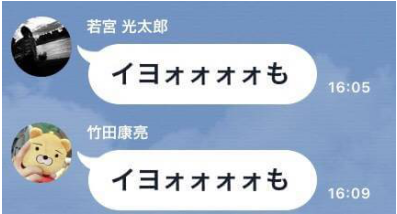
\includegraphics[clip,scale=0.5]{iii}
    \caption{小川男葉集III}
    \label{iii}
\end{figure}



\newpage
\subsubsection{小川男万葉集IV}
 \\
・アルステムダム\\
・オマンガンの鼻は犬\\
・広尾スタバ店\\
・スンマヒーンバッキンゴヒャクエンニナリマフー(交渉の余地なし)\\
・これで窪田美沙に投票するんやでぇトイレ\\
・公開固形(あつむ)\\
・なんかなああ(サイリウム)\\
・それではチェキのカウントダウンを始めます。5.4\\
    (2000円握りしめて)時間を止める\\
・結婚安泰 将来おめでとう\\
・非常に濃ゆい旅行であった\\
・インジビリブル\\
・次、オ・ガンマンのパアアン(ターン)\\
・シビリア鉄道\\
・よし。   \ \      え?\\
・まろやかさってパロメーター\\
・なにこのケンリツ(建立)\\
・タマンダンまだおるのかぁ(ATM)\\

\newpage
\subsubsection{小川男万葉集V}
・ミドルネーム何個あんの?\\
・あ、おれこの写真知らんわ(写っている)\\
・おれミツやわ、うぃ\\
・オガワポテンシャル、とうざい(到来)\\
・ひさやんバンバンビガロ(ひさやんレトリバー(レトリィバァ))\\
・山崎パルのハン祭(ポ)\\
・とうばらし(チェックイン)いや、軽い\\
・めっちゃ見たろう\\
・前田さんぶっ殺そう(ケータイ弄りながら)\\
・親指ちょっとでっかくして(Christoph Falk Anders)\\
・どういうモチベーションで生きたらいいん、差しコエ\\
・やすおこプンプン丸\\
・インストールできない実験にインストールできる(ティ)\\
・定量的には何もわかりません(ピ)\\
・本当にあってるかどうかはわからないんですが(ポ)\\
・擬ラピデティに関しましては、私はちょっと(マ)\\
・前回と比べると誤差は大きく小さくなったと言えます(マ)\\
・ペットボトル加速器\\
・パーラー\\
・ミートボール10個で100倍\\
・僕ミートボール\\
・1/16通り\\
・美容院には来週末で予定していたのでバサバサ頭が気になった。普段はもっと若々しくてハツラツとしてキレイにしてると友達に言っといてな\\


\newpage
\section{Clock Doraemon Threshold Valentien(CDTV)}
\subsection{オガワマワン(23)が結婚できない20の理由}
\subsubsection{オガワマワン(23)が結婚できない20の理由}
 \\
(1)収入が安定していない\\
(2)無職\\
(3)何かに追われている、余裕が無い\\
(4)休日はYouTubeを見ている\\
(5)地下アイドルに友達がいる\\
(6)4σを言い張る\\
(7)お酒が弱い\\
(8)財布を無くしがち\\
(9)芸人だから\\
(10)方向音痴だから\\
(11)Googleマップを使うのが下手くそ\\
(12)コンパイルがあんまり通らないあ\\
(13)希望新風が好きすぎる\\
(14)映画が好きじゃないから\\
(15)杉下右京が好きだから\\
(16)お腹が緩い\\
(17)ツッコミ過ぎる\\
(18)指が太い\\
(19)結婚指輪の制度を知らない\\
(20)結婚の意識が無い\\
(21)ボインボイン物語で喜ぶ\\
(22)天然だから\\
(23)土下座できない\\
\\
【説明】\\
この男はノリピーをこきおろしている。\\

\newpage
\subsubsection{オガワマワン(24)が結婚できない20の理由が冤罪である理由}
 \\
(1)社会人であるため安定している{\sf (´\_ゝ`)}笑\\
(2)社会人であるため無職ではない{\sf (´\_ゝ`)}笑\\
(3)追われていない、毎日工場実習で退屈な日々を過ごしている{\sf (´\_ゝ`)}笑\\
(4)そこまで見ていない、平日のほうが見ている{\sf (´\_ゝ`)}笑\\
(5)まあ知り合いといったところでしょうか{\sf (´\_ゝ`)}笑\\
(6)まあ5σ{\sf (´\_ゝ`)}笑\\
(7)弱いが嫌いではない{\sf (´\_ゝ`)}笑\\
(8)あれ以降なくしていない{\sf (´\_ゝ`)}笑\\
(9)芸人ではない{\sf (´\_ゝ`)}笑\\
(10)気のせい{\sf (´\_ゝ`)}笑\\
(11)Googleマップがバグっていただけ{\sf (´\_ゝ`)}笑\\
(12)コンパイルとか懐かしいな{\sf (´\_ゝ`)}笑\\
(13)海苔が好きなだけ{\sf (´\_ゝ`)}笑\\
(14)映画が好きじゃないわけではなく見る機会がないだけ{\sf (´\_ゝ`)}笑\\
(15)杉下右京が好きでもない{\sf (´\_ゝ`)}笑\\
(16)寒いのが悪い{\sf (´\_ゝ`)}笑\\
(17)ボケが多いだけ{\sf (´\_ゝ`)}笑\\
(18)指が太いとは思わない{\sf (´\_ゝ`)}笑\\
(19)制度とかあったっけ{\sf (´\_ゝ`)}笑\\
(20)ある{\sf (´\_ゝ`)}笑\\
(21)喜んだ記憶はない{\sf (´\_ゝ`)}笑\\
(22)天然ではない{\sf (´\_ゝ`)}笑\\
(23)できないことはない{\sf (´\_ゝ`)}笑\\
\\
【説明】\\
なんやこれ{\sf (´\_ゝ`)}笑\\


\newpage
\subsection{インビジブル天然巨乳である10の理由}
\begin{enumerate}
\item 財布を無くしたと喚き、2時間友人を捜索に付き合わせた結果、カバンから出てきた。
\item カードの1/19という使用期限の表記を見て、「平成19年1月」と記入した。
\item 極度の肩凝り。
\item macとディスプレイを繋いでいないのに、ディスプレイ側にポインターを持っていこうとしていた。
\item「旅費申請が出来ない! なんやねん、これ!」と憤っていたのに、実はパスワードの打ち間違いが原因であった。
\item 店長になろうとした
\item CERN出張の宿について話している時に「結局ホステスになりそう」と言った
\item ビジブル貧乳
\item 六甲道集合なのに、六甲に集合した。
\item macとディスプレイを繋いでいないのに、「いや、放電っぽい波形が」とほざき、ディスプレイ側にスライドを持っていこうとしていた。
\item 食器用洗剤と勘違いをして、オリーブオイルで食器を洗っていた。
\item 自らのオリーブオイルの過ちを、他人の過失として男葉集内で処理しようとした。
\end{enumerate}

\newpage
\subsection{理想の女性100の条件}
 \\
---------- 検索結果 ---------- \\
    澁川 ◯◯ *******  80\%\\
    横山 Yumi ******  10\%\\
    明石家さんま *** 10\%\\
    あき竹城 *********  1‰\\
---------------------------------\\
(1)性別が女\\
(2)日本人またはインド人\\
(3)性格が素晴らしい(自分の事をヨイショする)\\
(4)年齢は±5歳\\
(5)身長は0cm以上170cm以下\\
(6)お喋り(他愛もない会話ができる、まぁ喋らんくても良いんやけどな)\\
(7)オシャレ\\
(8)漢検4級以上持ってると良い\\
(9)センター試験も受験していると尚良い\\
(10)関西弁を喋ってくれると、萌える\\
(11)標準語は、イラッとする(そんな事無い)\\
(12)運動はできたほうが良い\\
(13)できれば陸上(そんな事は無い)\\
(14)できれば水泳(そんな事は無い)\\
(15)髪型は不問とする。髪質は要相談。\\
(16)貧乳  (A以下もしくはB以上)\\
(17)**体重カット**山崎さんより越智さん(強いて言うなら)\\
(18)**女優カット** 綾瀬はるか、石原さとみ以外(別に省いてもええよ)\\
(19)新垣結衣(まぁまぁまぁ)\\
(20)明石家さんま以外\\
(21)笑っている時、口を開いている(笑顔がステキ)\\
(22)歌唱力は和田アキ子以上、出来れば声量も和田アキ子\\
(23)メガネを掛けていないのが好ましい(あき竹城)\\
(24)タバコを吸わない\\
(25)体重は80kg以下\\
(26)ショートの方が良い(似合ってたら何でも良いけど)\\
(27)メンヘラ・束縛系は駄目(おれは束縛せぇへんから)\\
(28)大食いが好ましい\\
(29)山崎さんよりさんま\\
(30)徳永英明より高音域を歌える女性\\
(31)料理は好きで、自分よりちょっと上(パスタマシン保有)\\
(32)白い\\
(33)毛量は多いほうが好ましい、葉加瀬太郎\\
(34)Zカップ以下\\
(35)性格について俺から言うことは無い、ニートでも可\\
(36)脚が100cm、胴体60cm\\
(37)得意料理は和食であれば良い、スパイスの効いたカレーなら尚良。\\
(38)専業主婦でドM、首輪で飼いたい。\\
(39)早起き(4時起き)が良い\\
(40)インド\\
\\
-- reserved --\\ 
(65)チュエンティフォー\\
(80)胸が盆地\\
(89)未婚が望ましい\\
(100)自分の事がチュキダカラ(自分っておれやで)\\

\newpage
\subsection{オ・マンガンが女々しい10の理由}
\begin{enumerate}
\item 星野源が好きだから(アボカドはそこまで。)
\item .
\item .
\item .
\item .
\item .
\item .
\item .
\item .
\item .
\end{enumerate}


\subsection{オ・マンガンが男らしい10の理由}
\begin{enumerate}
\item .
\item .
\item .
\item .
\item .
\item .
\item .
\item .
\item .
\item .
\end{enumerate}

\newpage
\subsection{オ・マンガンがインド人かもしれない10の理由}
\begin{enumerate}
\item 顔がインド人(登校してすぐの発言)
\item 学部時代に英語でカバディを習得した。
\item 本名がガワッシュ・モハンマド
\item 好きなタイプがインド人
\item 牛より豚を食べる
\item タバコよりうんこ
\item ナマステ、と声を掛けられた。
\item .
\item .
\item .
\end{enumerate}

\subsection{オ・マンガンが前田健太かもしれない10の理由}
\begin{enumerate}
\item マエケン体操が上手い
\item .
\item .
\item .
\item .
\item .
\item .
\item .
\item .
\item .
\end{enumerate}

\newpage
\subsection{比叡比叡推進協会}
図\ref{gas1}に一覧を示す。

\begin{table}[htb]
\newcolumntype{C}{>{\centering}p{5em}}
\begin{center}
\begin{tabular}{|c|c|} 
\hline
	会長 & 小川圭将\tabularnewline  \hline
庶務 & 山下達郎\tabularnewline  \hline
東京支部長・人事部長 & 前川光輝\tabularnewline  \hline
幹事・忘年会隊長 & 越智敦彦\tabularnewline  \hline
補佐 & 藏重久弥\tabularnewline  \hline
環境保全対策長 & 小川圭将\tabularnewline  \hline
副総理 & 又吉硬木\tabularnewline  \hline
エンジニアリング部門隊長 & 村上ショージ\tabularnewline  \hline
環境保全部門 農園部隊隊長 & 小川圭将\tabularnewline  \hline
環境保全アセスメント部隊 & 解散\tabularnewline  \hline
失言訂正担当大臣 & 小川圭将\tabularnewline  \hline
迷子担当大魔王 & 小川圭将\tabularnewline  \hline
長野支部スキー本部長 & ニセヨンテ\tabularnewline  \hline
路面凍結防止部隊 & 若宮光太郎\tabularnewline  \hline
美声部門オーケストラ学科 & 美輪明宏\tabularnewline  \hline
自衛自衛部門安全保障学科 & 桜井誠\tabularnewline  \hline
医療部門心電図工作隊長 & 越智敦彦\tabularnewline  \hline
学長部門学長 &武田廣\tabularnewline 
	\hline
	\end{tabular}
	\end{center}
	\caption{比叡比叡推進協会}  
	\label{gas1}
\end{table}

\newpage
\subsection{オガワマンのあだ名一覧}
\begin{itemize}
\item オマゲン(12/21)
\item オマガンメン
\item オマンギョンボン号
\item オガワン・バンバ・バン
\item オゲンマン
\item オマンゲン・ゴン
\item オマンゲン
\item オマンゲンゴンガングン
\item オガコウモン
\item オ・ヨンジュン
\item バラタン星人
\item オマンゲン源マン
\item オマンゲングンソクバン
\item 宮崎マン
\item オガワ3
\item オゾンマン
\item オズ
\item オズモ
\item オザワ
\item オマンゲンゴンガンバ
\item オザンギン
\item On the rock
\item オガンディー
\item オガァァァバン
\item 御万願寺
\item クルシウス小川
\item オマンゲン
\item 世界のオギャワ
\item オガワン星人
\item オガワン・バンバン・ビガロ
\item オガワン・オガワ
\item オガワン・ババン・バンバンバン
\item おがパイオン
\item おーゆー
\item 湯川
\item オガワン・ケノービー
\item オガワのマンメン
\end{itemize}


\newpage
\chapter{まとめ}
Some implications and consequences of the expansion of the universe are examined. In Chapter 1 it is shown that this expansion creates grave difficulties for the Hoyle-Narlikar theory of gravitation. Chapter 2 deals with perturbations of an expanding homogeneous and isotropic universe. The conclusion is reached that galaxies cannot be formed as a result of the growth of perturbations that were initially small. The propagation and absorption of gravitational radiation is also investigated in this approximation. In Chapter 3 gravitational radiation in an expanding universe is examined by a method of asymptotic expansions. The 'peeling off' behaviour and the asymptotic group are derived. Chapter 4 deals with the occurrence of singularities in cosmological models. It is shown that a singularity is inevitable provided that certain very general conditions are satisfied.\\
 A very large scintillating fiber (SciFi) tracking detector for the K2K long baseline neutrino oscillation experiment has been in operation since March, 1999. Track finding efficiency is 98±2 \% for long muon tracks (those which intersect more than 5 fiber planes), and 85±6 \% for short tracks, which were estimated using cosmic-ray muons and a Monte Carlo simulation. The position resolution per layer is about 0.8 mm. The SciFi detector has demonstrated its capability for reconstruction of νμ interactions. The pulse heights for cosmic- ray muons have been stable within 10 \% after one year of operation. In addi- tion, the SciFi detector offers the possibility of performing electron and proton identification.\\
 Christoph is a postdoc at the University of Heidelberg’s physics institute in Germany. He has been working in ATLAS since 2007. His research is currently focussed on the identification of very energetic heavy particles, e.g. top quarks. When he is not looking for physics beyond the Standard model, he likes reading, listening to music, photography, cooking, traveling with his wife, playing board games with friends and sports.



テスト\cite{Aad:2012tfa}

\bibliographystyle{junsrt}
\bibliography{ref}

\end{document}
